% \begin{savequote}[8cm]
% Alles Gescheite ist schon gedacht worden.\\
% Man muss nur versuchen, es noch einmal zu denken.

% All intelligent thoughts have already been thought;\\
% what is necessary is only to try to think them again.
%   \qauthor{--- Johann Wolfgang von Goethe \cite{von_goethe_wilhelm_1829}}
% \end{savequote}

\chapter{\label{ch:2-neutrinophysics}Neutrino physics}

\minitoc

This chapter includes a brief historical overview and a review of the introductory theoretical background of neutrino physics. In particular, the mechanism of neutrino oscillations will be described and several neutrino experimental anomalies will be reviewed. The constraints and the hints for additional, non-weakly interacting neutrino states from neutrino experiments, will also be presented.

\section{Introduction}

Neutrino physics represents one of the most exciting areas of active research in particle physics. The history of the early days of particle physics shows that neutrinos have challenged physicists since the famous Pauli's letter to his fellow \emph{Radioactive Ladies and Gentlemen} \cite{Pauli:1930pc}, where he postulated the existence of a new neutral particle to explain the continuous spectrum of the nuclear $\beta$-decay.  Fermi hypothesised the neutrino to be emitted in the three-body process:
\begin{equation}
    n\rightarrow p + e^{-} + \bar{\nu}_{e},
\end{equation}
and mediated by a four-fermion interaction in the form of:
\begin{equation}
    \frac{G_{F}}{\sqrt{2}}(\bar{n}\Gamma_{N}p)(\bar{\nu}_{e}\Gamma_{L}e),
\end{equation}
where, in modern terms, $G_{F}$ is the Fermi constant and $\Gamma_{N,L}$ are a linear combination of the \emph{gamma matrices}. The Feynman diagram of the four-fermion approximation of $\beta$-decay is shown in Figure \ref{fig:fermibeta}.

\begin{figure}
    \centering
    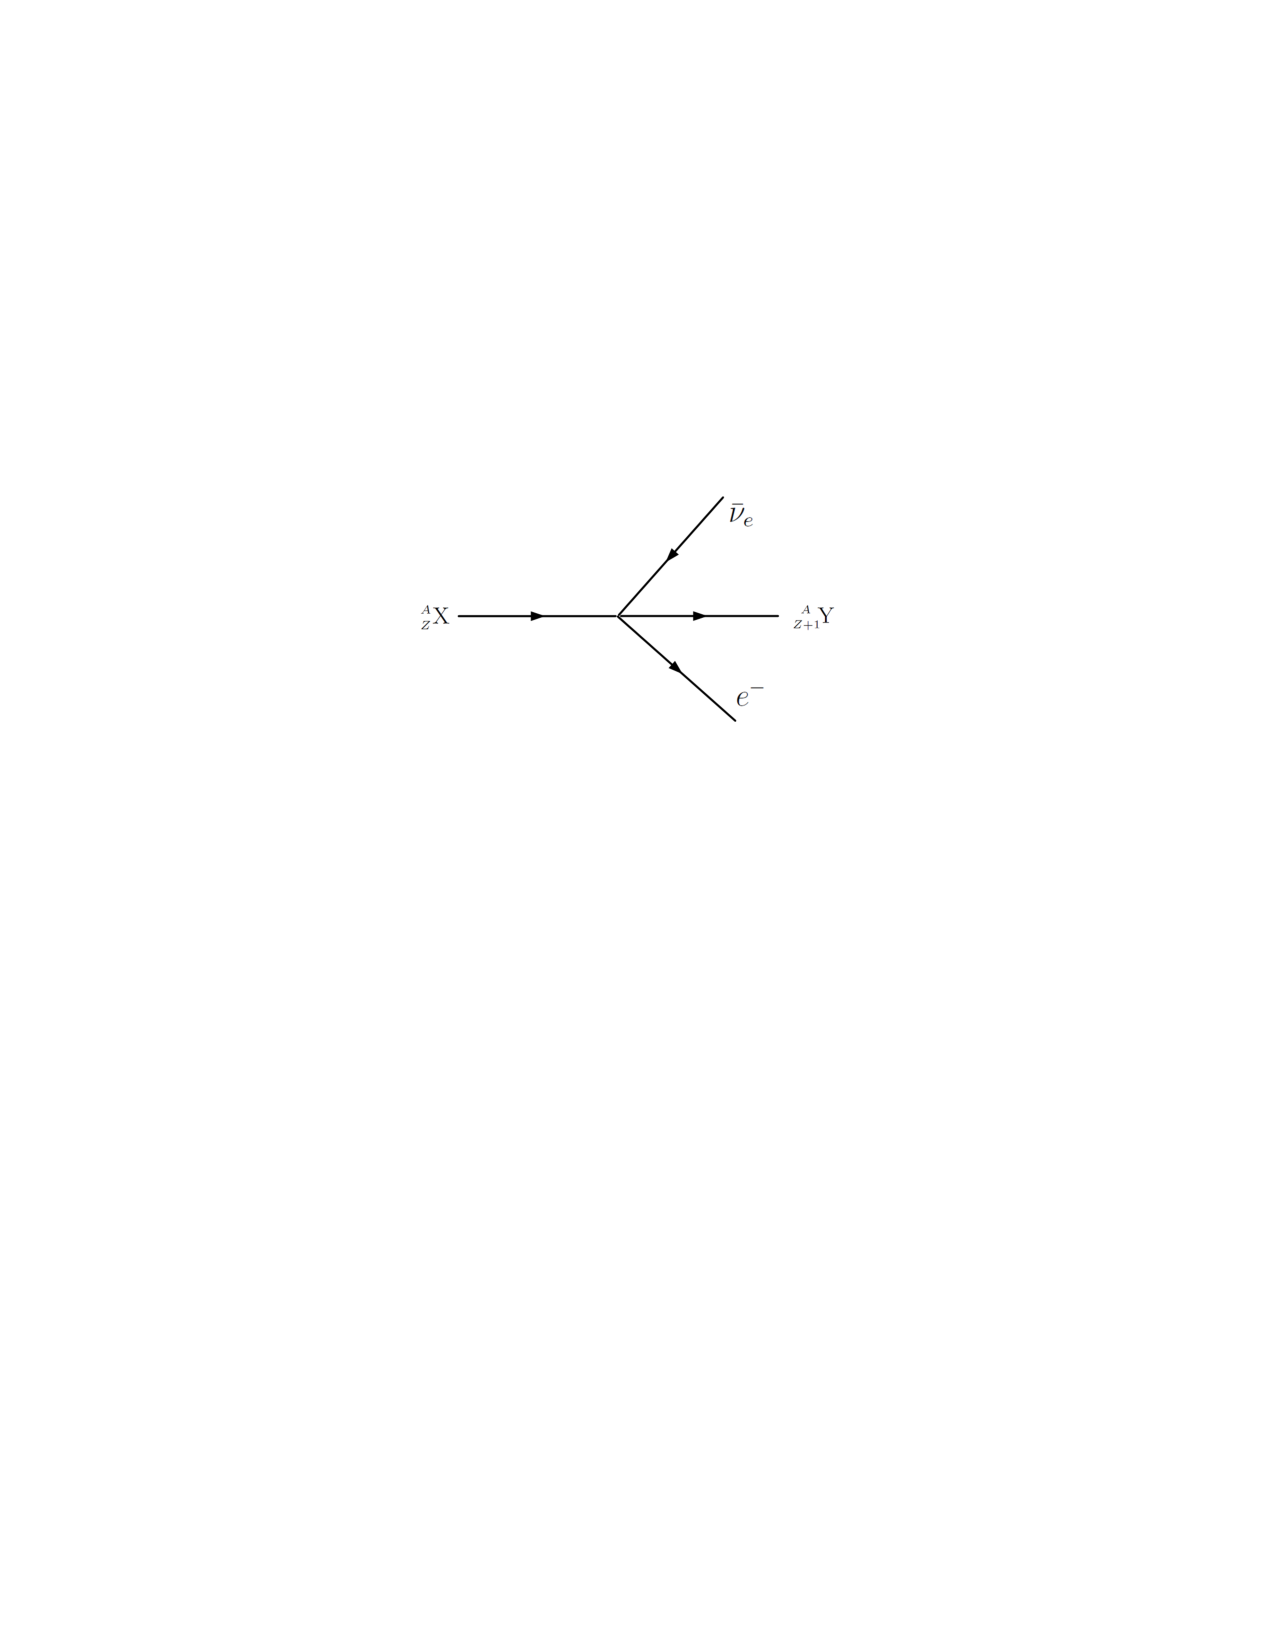
\includegraphics[width=0.7\linewidth]{figures/fermidecay.pdf}
    \caption{Feynman diagram of the $\beta$-decay of a $^{A}_{Z}X$ into a $^{A}_{Z+1}Y$ nucleus in the Fermi approximation.}
    \label{fig:fermibeta}
\end{figure}

This theory paved the way for the first experimental direct detection of neutrinos by Cowan and Reines in 1956 \cite{Cowan:1992xc}, which exploited the inverse $\beta$-decay process:
\begin{equation}
    \bar{\nu}_{e} + p \rightarrow e^{+} + n.
\end{equation}
The key detection technique, still used in modern reactor experiments, employed the detection of the $e^{+}e^{-}\rightarrow 2\gamma$ annihilation and the $\gamma$ emitted by the capture of the recoiling neutron shortly afterwards. 

The leptonic current $\bar{\nu}_{e}\Gamma_{L}e$ was later hypothesised to be left-handed in the form of $\gamma_{\mu}(1-\gamma_{5})$ ($V-A$) by Feynman and Gell-Mann \cite{Feynman:1958ty}.
For massless neutrinos this allows to assign a left-handed (right-handed) helicity to neutrinos (anti-neutrinos), which was experimentally verified by Goldhaber \cite{Goldhaber:1958nb}.

\section{Neutrino Oscillations Theory}
In the modern Standard Model of particle physics there are three flavours of (anti)neutrinos ($\nu_{e}$, $\nu_{\mu}$, $\nu_{\tau}$), each one paired to a charged (anti)lepton ($e$, $\mu$, $\tau$ respectively). 
However, if neutrinos have masses, it is possible to have three (or more) neutrino mass eigenstates ($\nu_{1}$, $\nu_{2}$, $\nu_{3}$, ...) analogues of the charged-lepton mass eigenstates. 
In this case, a neutrino produced as a flavour eigenstate would \emph{oscillate} through its path and change to another flavor eigenstate. This happens because the flavour eigenstate is a mixture of the three (or more) mass eigenstates, which travel with different wavelengths and create interference patterns. 

The oscillation probabilities can be derived in the case of two neutrino generations, which we report here for didactic reasons largely following the approach in \cite{deGouvea:2004gd}. The flavour eigenstates $\nu_{\alpha}, \nu_{\beta}$ can be expressed as a superposition of the two mass eigenstates $\nu_1$ and $\nu_2$ using the nominal rotation matrix $U$:
\begin{equation}
U = \begin{bmatrix}
    \cos\theta & -\sin\theta \\
    \cos\theta & \sin\theta
    \end{bmatrix}.
\end{equation}

The flavour neutrino $\nu_{\alpha}$ will then propagate as: 
\begin{equation}
    \ket{\nu_{\alpha}} = \cos\theta\ket{\nu_{1}}+\sin\theta\ket{\nu_{2}}
\end{equation}

The time evolution of this superposition can be written, in the plane-wave assumption, as:
\begin{equation}
    \ket{\nu(\vec{x},t)} = \cos\theta e^{-ip_{1}x}\ket{\nu_{1}}+\sin\theta e^{-ip_{1}x}\ket{\nu_{2}}.
\end{equation}
If the neutrino is ultra-relativistic the exponential argument becomes:
\begin{equation}
\begin{split}
    p_{i}x & = E_{i}t - \vec{p}_{i}\vec{x} \simeq (E_{i}-p_{z,i})L\\
           & = (E_{i}^2-|\vec{p}|^{2})/(E_{i}-p_{z,i})L\\
           & \simeq m_i^{2}/2E_{i}L \simeq m_i^{2}/2E L,
\end{split}
\end{equation}
and the oscillation probability of the neutrino with flavour $\alpha$ can be written as:
\begin{equation}
\begin{split}
    P_{\alpha\alpha} & = |\bra{\nu_{\alpha}}\ket{\nu(L)}|^2\\
                     & = 1 - \sin^2 2\theta \sin^2\left(\frac{\Delta m^{2}L}{4E}\right),\label{eq:prob}
\end{split}
\end{equation}
where $\Delta m^{2} \equiv m^2_2-m^2_1$ is the mass splitting between the two mass states at play. The probability of observing a neutrino of flavour $\beta$ will be then given by:
\begin{equation}
    P_{\alpha\beta} = 1 - P_{\alpha\alpha} = \sin^2 2\theta \sin^2\left(\frac{\Delta m^{2}L}{4E}\right).\label{eq:prob2}
\end{equation}
Eq. \eqref{eq:prob} and \eqref{eq:prob2} show that the amplitude of the oscillation is regulated by the rotation angle $\theta$, while its frequency depends on the mass splitting, at a fixed $L/E$ ratio. Figure \ref{fig:oscillation} shows as an example the $\nu_e$ survival probability as a function of the neutrino energy for $L=180$~km, $\Delta m^2 = 7.0 \times 10^-5$~ev$^2$ and $\sin^2\theta = 0.84$. 

\begin{figure}
    \centering
    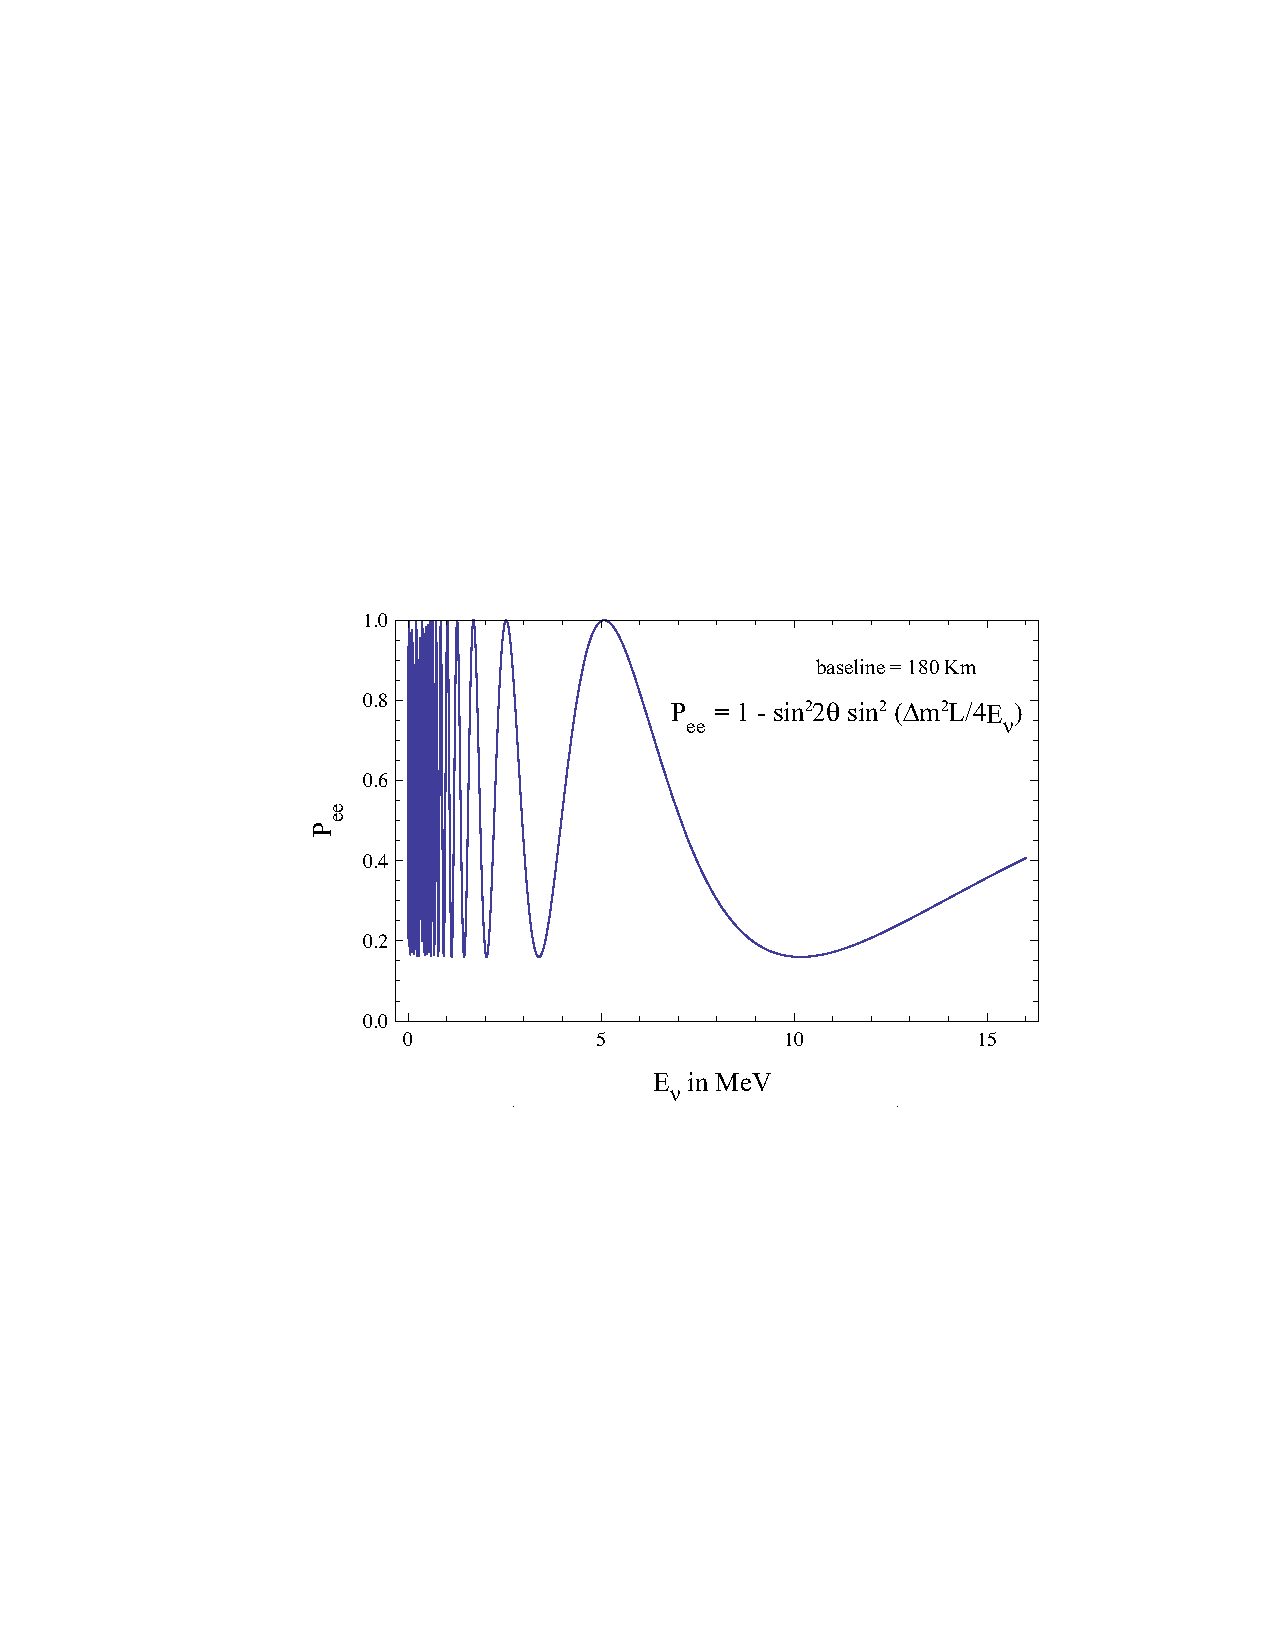
\includegraphics[width=0.7\linewidth]{figures/oscillation.pdf}
    \caption{The $\nu_e$ survival probability $P(\nu_e\rightarrow\nu_e)$ as a function of the neutrino energy for $L=180$~km, $\Delta m^2 = 7.0 \times 10^-5$~ev$^2$ and $\sin^2\theta = 0.84$.}
    \label{fig:oscillation}
\end{figure}

Neutrino oscillations experiments can be divided into two main categories: \emph{disappearance experiments}, which measure the deficit of neutrinos of a certain flavour (measuring $P_{\alpha\alpha}$), and \emph{appearance experiments}, which look for an excess of neutrinos of a certain flavour (measuring $P_{\alpha\beta}$).

The $U$ matrix can be easily extended in the case of the three generations of neutrinos $\nu_{e}$, $\nu_{\mu}$, and $\nu_{\tau}$. In this case, the flavour eigenstates mixing is obtained from:
\begin{equation}
\begin{bmatrix}
\nu_{e}\\
\nu_{\mu}\\
\nu_{\tau}
\end{bmatrix}=
\begin{bmatrix} U_{e 1} & U_{e 2} & U_{e 3} \\ U_{\mu 1} & U_{\mu 2} & U_{\mu 3} \\ U_{\tau 1} & U_{\tau 2} & U_{\tau 3} 
\end{bmatrix} 
\begin{bmatrix} \nu_1 \\ \nu_2 \\ \nu_3 \end{bmatrix},
\end{equation}
where the rotation is given by the so-called Pontecorvo–Maki–Nakagawa–Sakata (PMNS) matrix. It is also possible to parametrise the $U$ matrix in the following useful way:
\begin{align} 
  U_{\mathrm{PMNS}} = \begin{bmatrix} 1 & 0 & 0 \\ 0 & c_{23} & s_{23} \\ 0 & -s_{23} & c_{23} \end{bmatrix}
 \begin{bmatrix} c_{13} & 0 & s_{13}e^{-i\delta_{CP}} \\ 0 & 1 & 0 \\ -s_{13}e^{i\delta_{CP}} & 0 & c_{13} \end{bmatrix}
 \begin{bmatrix} c_{12} & s_{12} & 0 \\ -s_{12} & c_{12} & 0 \\ 0 & 0 & 1 \end{bmatrix},\label{eq:pmns}
\end{align}
where  $s_{ij}$ ($c_{ij}$) is an abbreviation for $\sin\theta_{ij}$ ($\cos\theta_{ij}$) and $\delta^{CP}$ is the CP-violating phase. The mixing angles $\theta_{12}$, $\theta_{13}$, and $\theta_{23}$ are defined by:
\begin{equation}
    \tan^2\theta_{12}\equiv\frac{|U_{e2}|^2}{|U_{e1}|^2},\quad
    \tan^2\theta_{23}\equiv\frac{|U_{\mu3}|^2}{|U_{\tau3}|^2},\quad
    \sin\theta_{13}\equiv U_{e3}e^{i\delta^{CP}}.
\end{equation}

With three neutrino flavours the squared mass-splitting terms are $\Delta m_{12}^2$ and $\Delta m_{13}^2$. This cause a degeneracy in the ordering of three masses: it is possible to have $m_3 > m_2 > m_1$ (\emph{normal hierarchy}) or $m_3 > m_1 > m_2$ (\emph{inverted hierarchy}). Customarily, $\Delta m_{12}^2$ and $\Delta m_{13}^2$ are also called $(\Delta m^2)_{\mathrm{sol}}$ and $(\Delta m^2)_{\mathrm{atm}}$, respectively, since they are usually measured with "solar" and "atmospheric" neutrinos. The situation is illustrated in Figure \ref{fig:masshierarchy}, adapted from \cite{Cahn:2013taa}.

\begin{figure}
    \centering
    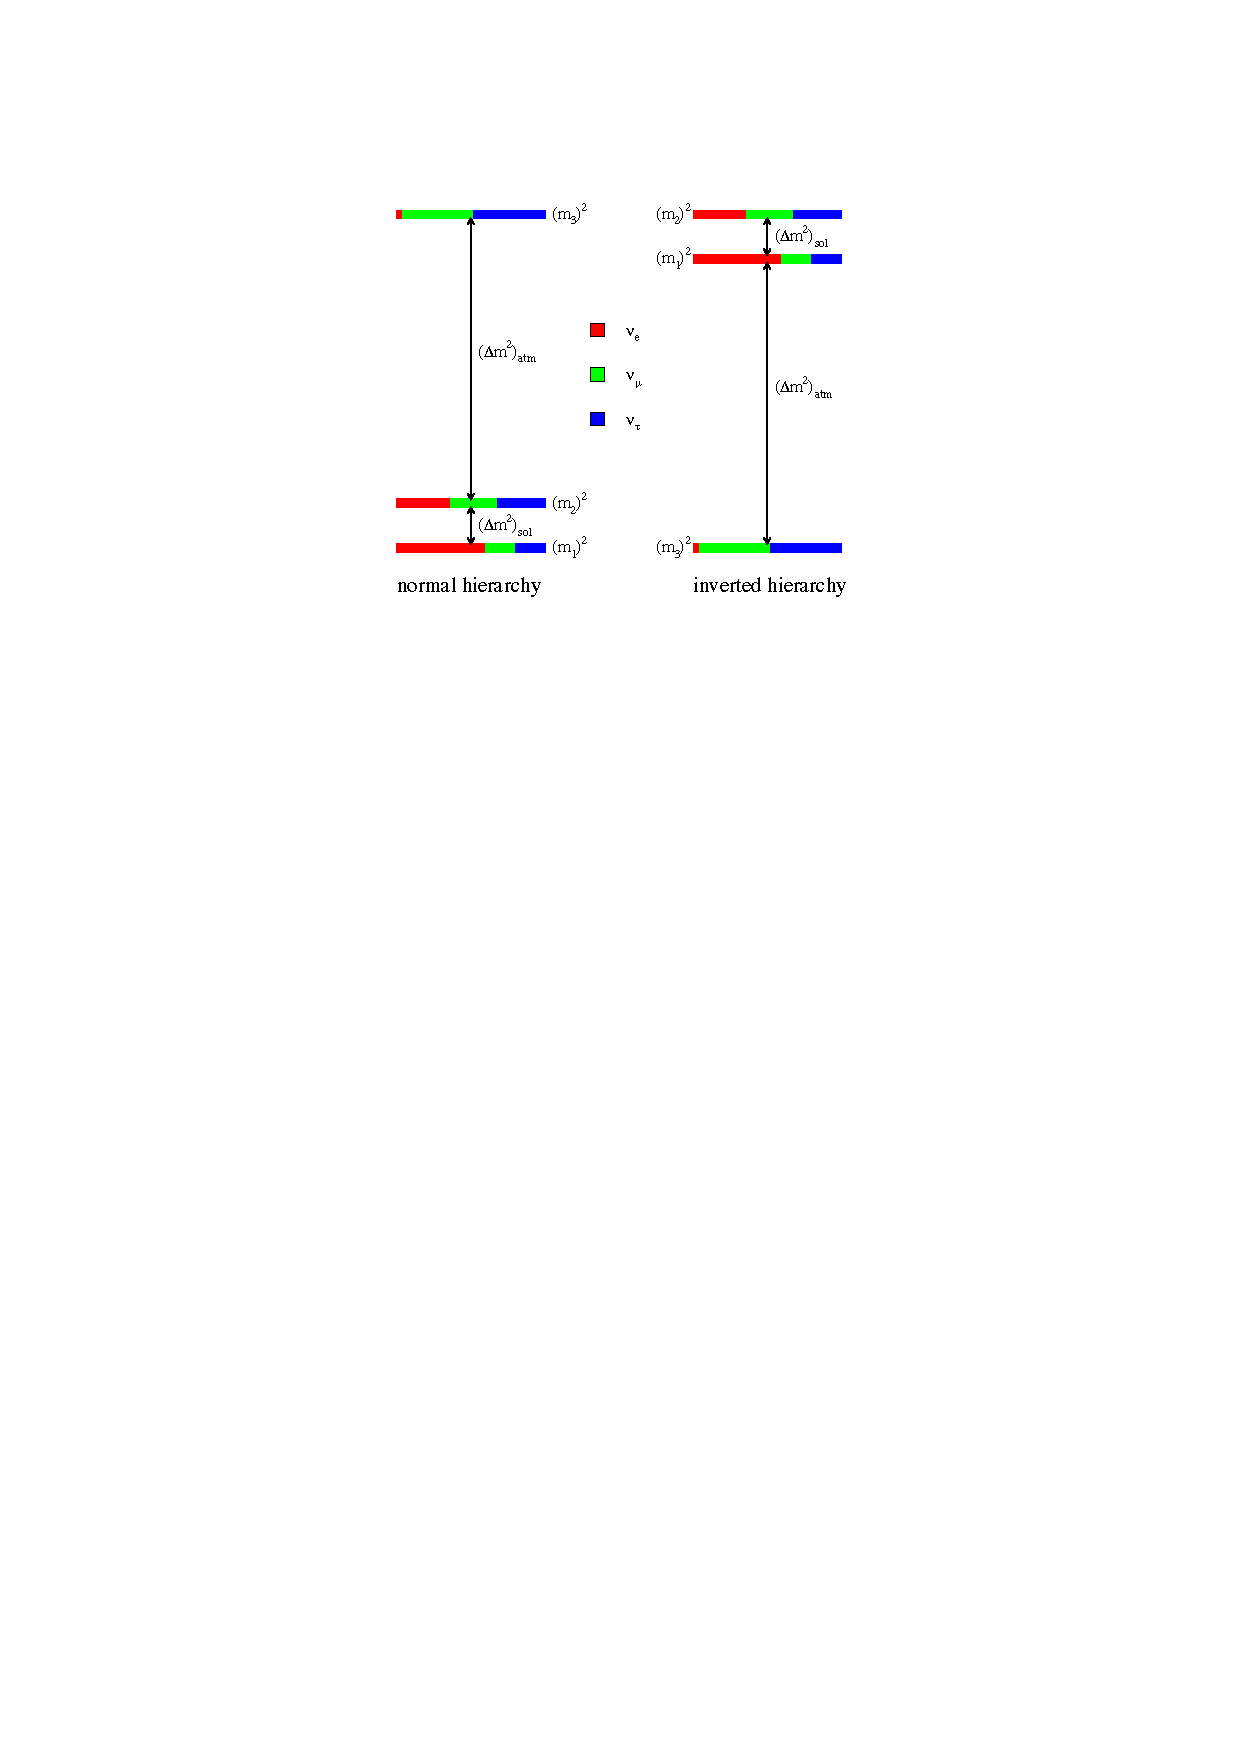
\includegraphics[width=0.75\linewidth]{figures/masshierarchy.pdf}
    \caption{Diagram of the normal and inverted hierarchies. The colours correspond to the fraction of each distinct flavor contained in the mass eigenstate.}
    \label{fig:masshierarchy}
\end{figure}

The mass splittings also determine the $L/E$ ratio at which the oscillation probability is maximised. In the assumption of two-neutrino oscillation, the oscillation frequency in eq. \eqref{eq:prob} becomes:
\begin{equation}
     \frac{\Delta m^{2}L}{4E} = 1.267\left(\frac{L}{\mathrm{km}}\right)\left(\frac{\Delta m^2}{\mathrm{eV}^2}\right)\left(\frac{\mathrm{GeV}}{E}\right),
\end{equation} 
which gives for $\theta_{12}$, $\theta_{13}$, and $\theta_{23}$ a maximum oscillation probability at $\approx 10^4$~km/GeV, $\approx 10^2$~km/GeV, and $\approx 10^2$~km/GeV, respectively. For this reason, $\theta_{12}$, $\theta_{13}$, and $\theta_{23}$ are also known as the \emph{solar}, \emph{reactor}, and \emph{atmospheric} mixing angles. In the parametrisation of the $U_{\mathrm{PMNS}}$ matrix of eq. \eqref{eq:pmns}, the product of the matrices can then be written as:
\begin{equation}
    U_{\mathrm{PMNS}} = U_{\mathrm{atm}} \cdot U_{\mathrm{reactor}} \cdot U_{\mathrm{sol}}.
\end{equation}



\section{Experimental Evidence of Neutrino Oscillation}
After the first direct detection of electron (anti)neutrinos by Cowan and Reines at the Savannah nuclear reactor \cite{Cowan:1992xc}, efforts were made in order to observe the other two neutrino flavours.
In 1962, Lederman and others \cite{PhysRevLett.9.36} first saw evidence of muon neutrinos interacting in the target and producing muons, while the DONUT collaboration finally observed the $\nu_{\tau}$ in 2001 \cite{Kodama:2000mp}.
However, the amount of neutrino interactions observed by several experiments was in disagreement with the one predicted by the theory of three massless neutrinos. In particular, two types of anomalies were identified, one involving the detection of solar neutrinos and one involving the neutrinos produced by cosmic rays in the atmosphere.

\paragraph{Solar neutrino anomaly}
The experiment by Ray Davis and others at Homestake was the first to directly detect the neutrinos produced in the sun \cite{Davis:1968cp}. However, the number of solar neutrino interactions was lower than expected and this deficit was later confirmed by several other experiments, including the Kamioka Observatory in Japan, the SAGE experiment in Russia, and the GALLEX experiment in Italy. The SNO (Sudbury Neutrino Observatory) experiment finally proved in 2001 that the cause of the deficit was the oscillation of the solar neutrinos into a different flavour eigenstate, by measuring both the solar $\nu_{e}$ flux and the total solar neutrino flux, as shown in Figure \ref{fig:sno} \cite{Ahmad:2002jz}. 

\begin{figure}[htbp]
    \centering
    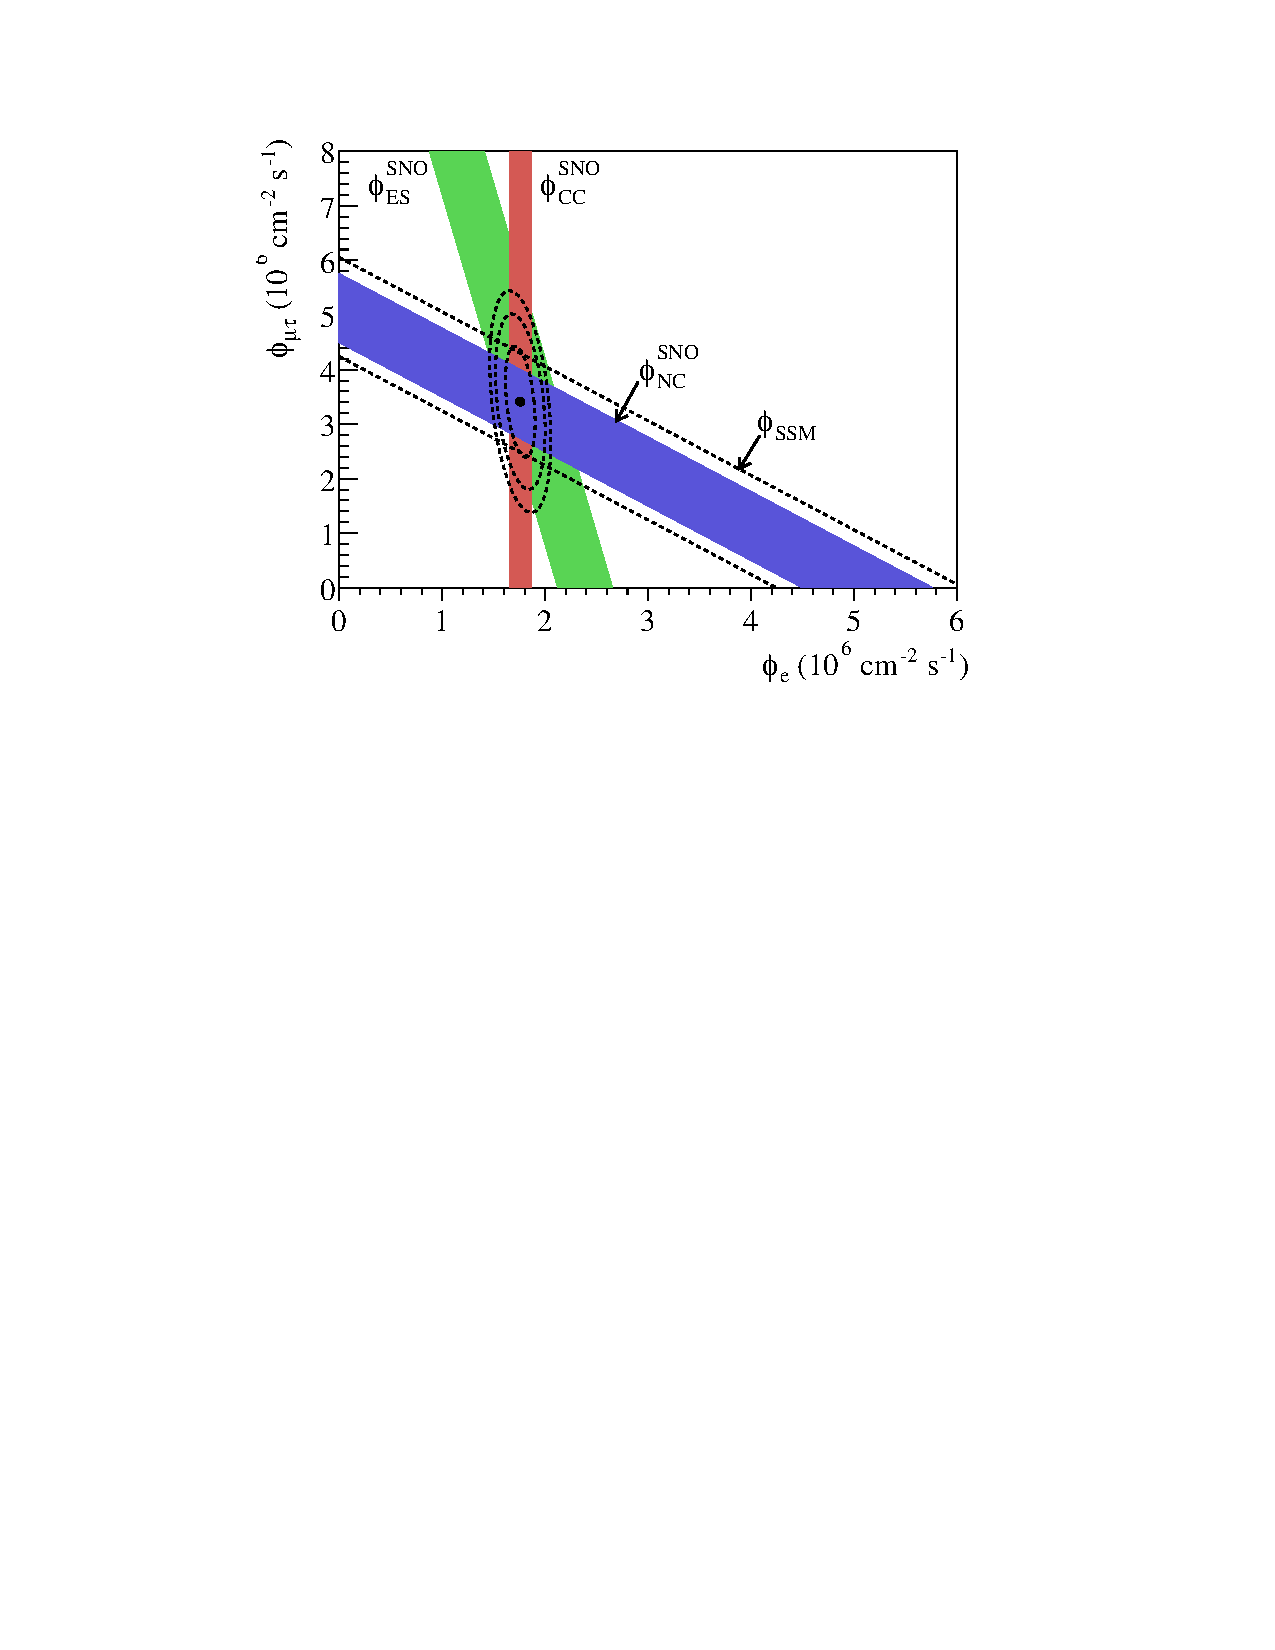
\includegraphics[width=0.7\linewidth]{figures/sno_plot.pdf}
    \caption{SNO measurement of the neutral-current ($\phi_{\mathrm{NC}}$), charged-current ($\phi_{\mathrm{CC}}$), and elastic scattering ($\phi_{\mathrm{ES}}$) fluxes. The CC measurement is sensitive to the $\nu_e$ flavour only, while the NC and ES fluxes depend both on $\nu_e$ and $\nu_{\mu}$/$\nu_{\tau}$ interactions. The neutrino flux predicted by the SSM (Standard Solar Model) is given by $\phi_{\mathrm{SSM}}$.}
    \label{fig:sno}
\end{figure}

The propagation of neutrinos in the matter is also determined by the Mikheyev-Smirnov-Wolfenstein (MSW) effect: in presence of a high density of electrons, electron neutrinos experience a charged current coherent forward scattering. This cause the electron neutrinos to have a different effective mass when they propagate in a high-density medium, modifying the oscillation pattern. 

The MSW effect is particularly important to explain the solar neutrino flux (Figure \ref{fig:solar}). Assuming a very high electron density in the sun core and an exponentially decreasing abundance (which are both good approximations in the standard solar model), the probability to observe an electron neutrino when it reaches the Earth is $P_{ee} \approx \sin^2\theta$ for neutrinos above 2~MeV (where the matter effect dominates).

\begin{figure}[htbp]
    \centering
    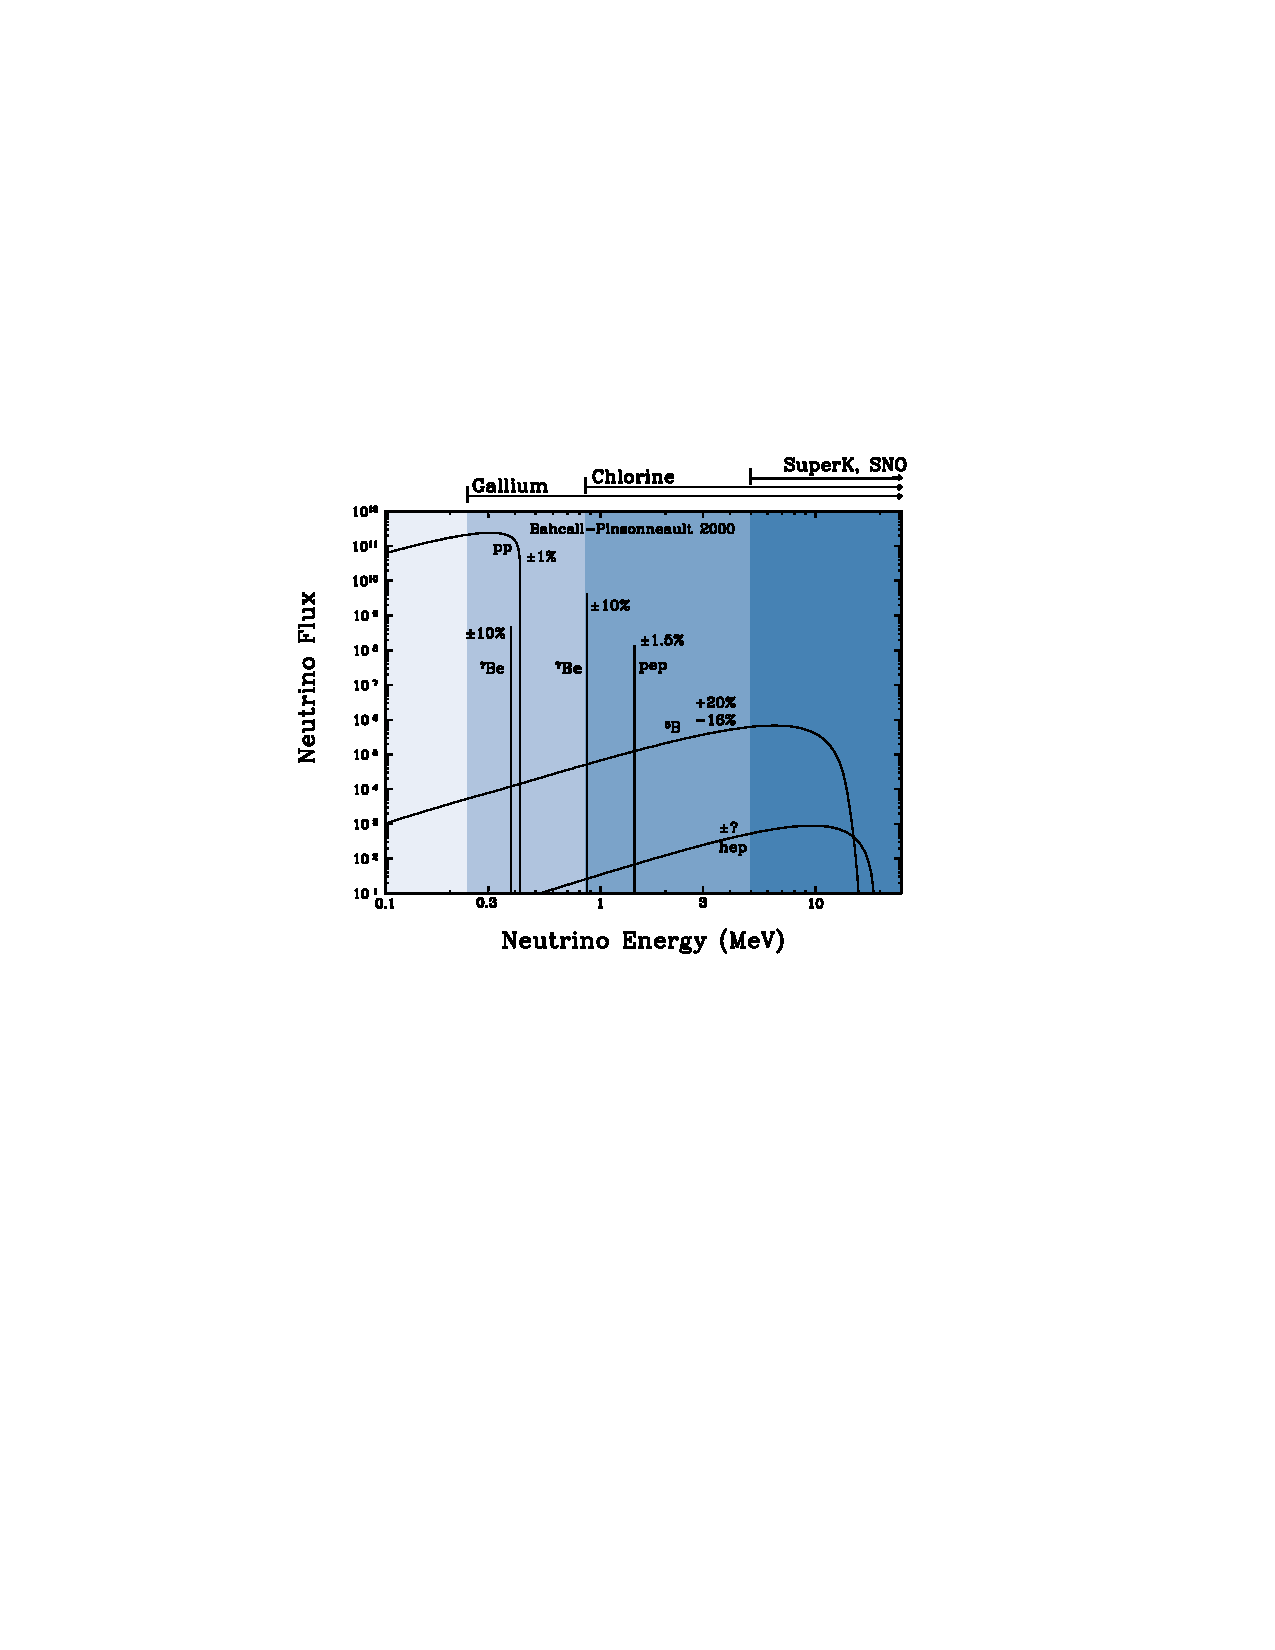
\includegraphics[width=0.75\linewidth]{figures/solar.pdf}
    \caption{The solar neutrino energy spectrum predicted by the solar standard model. Adapted from \cite{Bahcall:2000nu}.}
    \label{fig:solar}
\end{figure}

\paragraph{Atmospheric neutrino anomaly}
Cosmic muons decaying in the atmosphere produce a broad flux of muon (antineutrinos). The first underground water Cherenkov detectors, the IMB experiment and the Kamioka observatory, observed a discrepancy in the double ratio of muon to electron neutrinos, measured to expected. The evidence that this discrepancy was caused by the disappearance of atmospheric neutrinos was provided by the Super-Kamiokande experiment in 1998 \cite{Fukuda:1998mi}.

Figure \ref{fig:superk} shows the zenith angle distributions of events detected by the Super-Kamiokande experiment: the data points are in disagreement with the no-oscillation model and they can be interpreted as $\nu_{\mu} \leftrightarrow \nu_{\tau}$ oscillation.

In honour of these discoveries, the Nobel Prize in Physics 2015 was awarded to Takaaki Kajita (Super-Kamiokande) and Arthur B. McDonald (SNO). 

\begin{figure}[htbp]
    \centering
    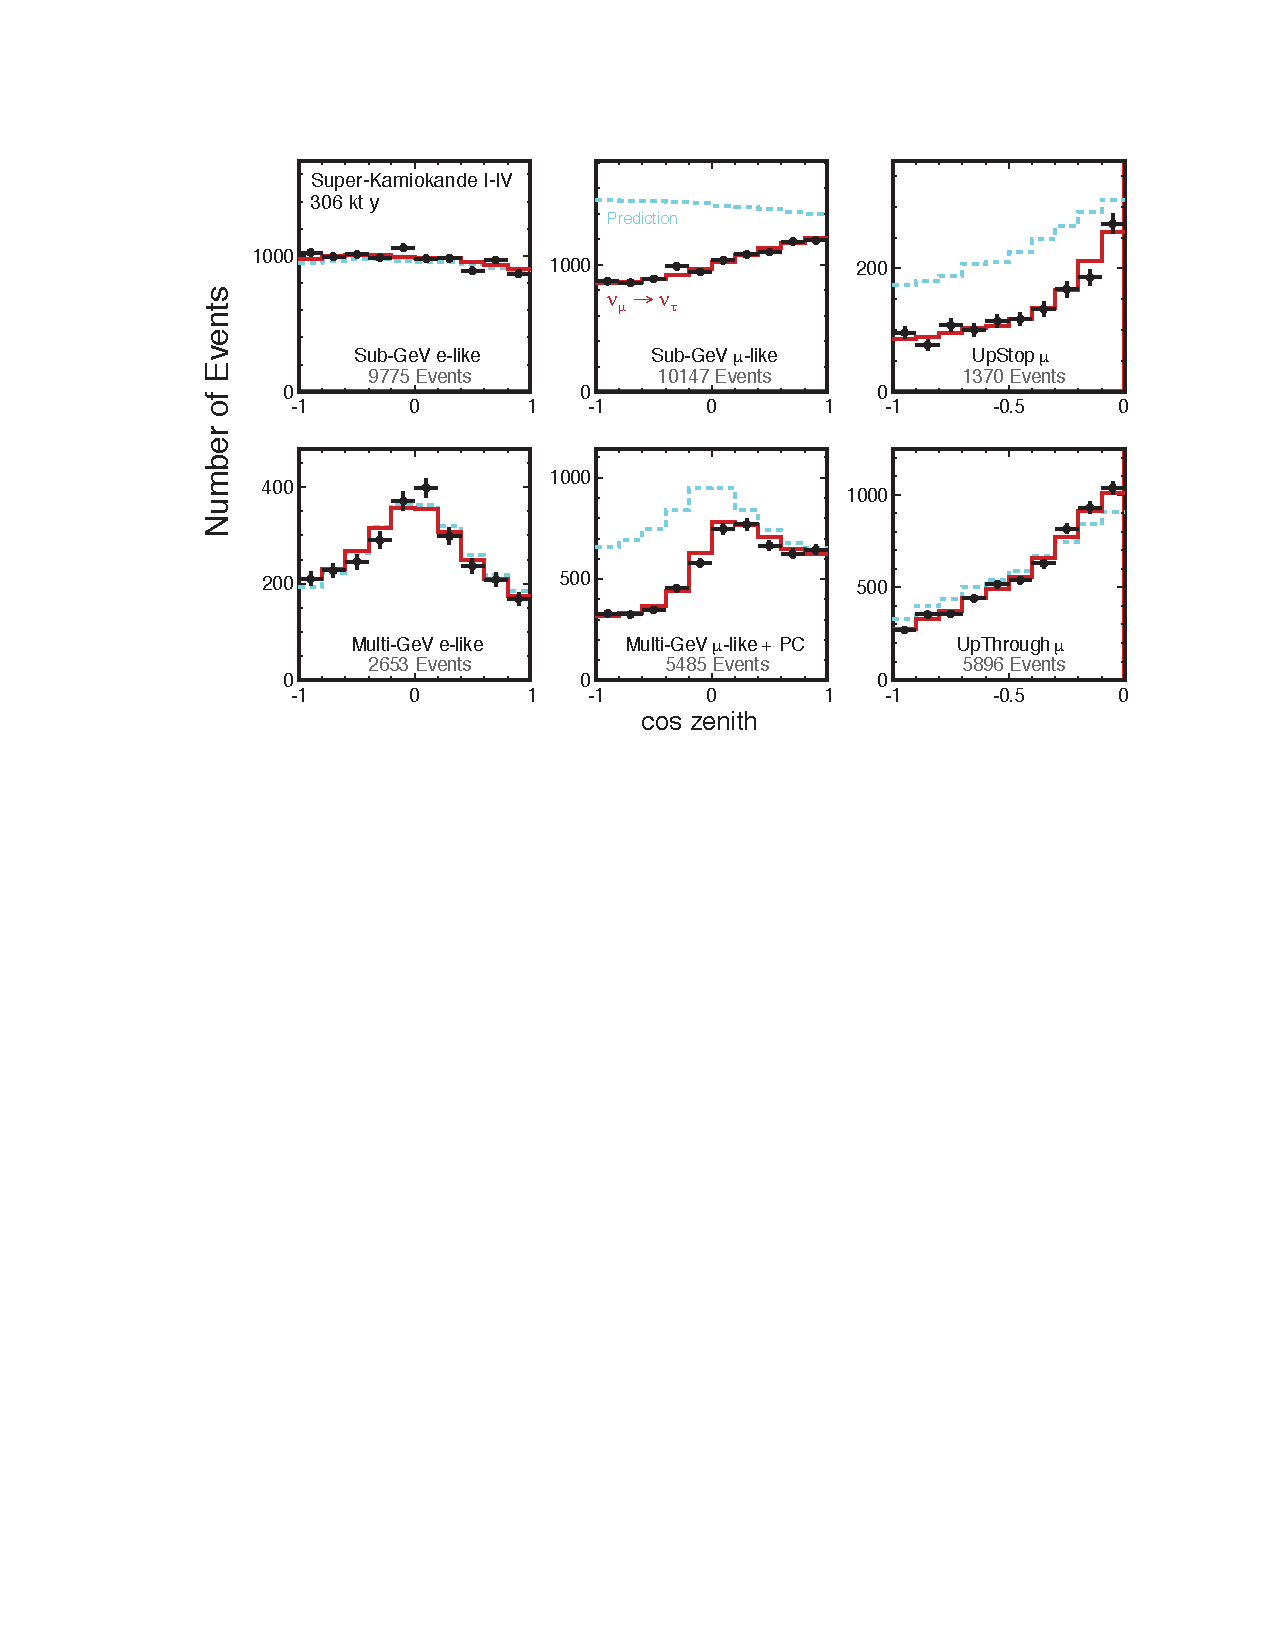
\includegraphics[width=0.9\linewidth]{figures/superk.pdf}
    \caption{Zenith angle distributions of $\mu$-like and e-like events in the sub-GeV and multi-GeV data sets, as collected by the Super-Kamiokande experiment. The dashed blue line corresponds to the no-oscillation model. The red solid line represent the best fit to $\nu_{\mu} \leftrightarrow \nu_{\tau}$ oscillation. Adapted from \cite{PhysRevD.98.030001}.}
    \label{fig:superk}
\end{figure}

\vspace{1em}

The KamLAND experiment finally spectacularly proved the oscillation pattern and the MSW model by measuring the reactor electron antineutrinos survival probability as a function of $L/E$, shown in Figure \ref{fig:kamland}. 

\begin{figure}[htbp]
    \centering
    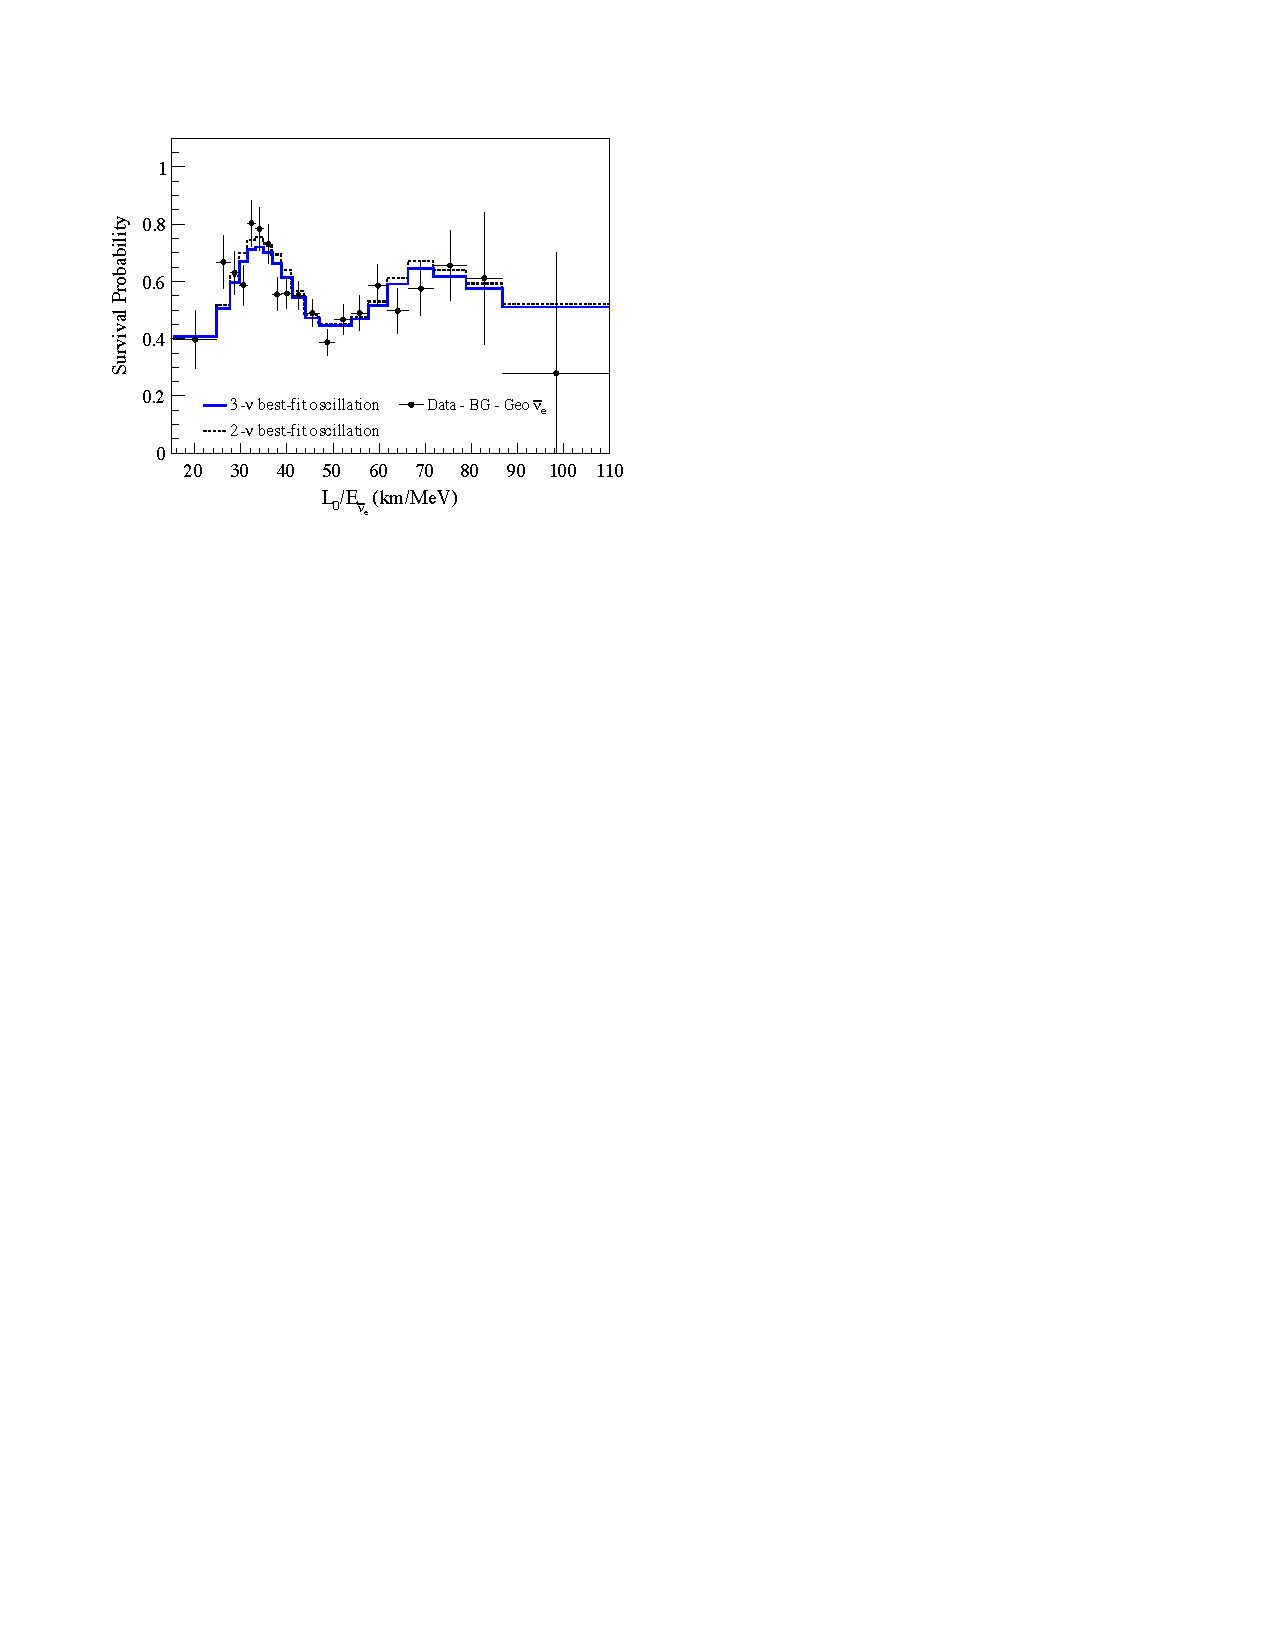
\includegraphics[width=0.75\linewidth]{figures/kamland.pdf}
    \caption{Ratio of the observed $\bar{\nu}_{e}$ spectrum to the expectation for no-oscillation versus $L_{0}/E$ for the KamLAND data. $L_{0} = 180$~km is the flux-weighted average reactor baseline. Adapted from \cite{Gando:2010aa}.}
    \label{fig:kamland}
\end{figure}

Less than 20 years after the definitive confirmation of neutrino oscillations, the mixing angles and the mass splittings are all known with a relative uncertainty smaller than 5\%. The least-known parameter in the PMNS matrix is the $\delta_{CP}$ phase, which, if different from $0^{\circ}$ (or from $180^{\circ}$), would imply CP-violation in the leptonic sector. This parameter can be measured only with appearance experiments, where it is possible to verify if
$P(\nu_{\alpha}\rightarrow\nu_{\beta}) \neq P(\bar{\nu}_{\alpha}\rightarrow\bar{\nu}_{\beta})$. Recent results from the T2K and NOVA experiments give a best fit of $\delta_{CP}/^{\circ}=215^{+40}_{-28}$ \cite{Esteban:2018azc}. A definitive measurement of the CP-violating phase would have far-reaching consequences in particle physics and cosmology, since it could explain the matter-antimatter asymmetry and provide an experimental basis for the leptogenesis model \cite{Fukugita:1986hr}.

A precise estimation of the MSW effect is particularly important for a correct measurement of the CP violation. Since the matter contains electrons and not positrons, the electron neutrinos will experience a MSW effect opposite to the one experienced by antineutrinos. This difference will, in turn, modify the appearance probabilities, leading to $P(\nu_{e}\rightarrow\nu_{\mu}) \neq P(\bar{\nu}_{e}\rightarrow\bar{\nu}_{\mu})$. This effect must the be disentangled from the CP-violating effect caused by the complex phases in the PMNS matrix.

The MSW effect is also dependent on the sign of the mass splitting $\Delta m_{31}$, which offers a way to resolve the hierarchy problem \cite{Smirnov:2013cqa}. 
In this document, however, we will focus on short-baseline neutrino experiments, where the MSW effect is negligible.

The number of \emph{light} neutrino species (meaning $m_{\nu} < m_{Z}/2$) weakly interacting was also determined by precision measurements of the $Z$ boson width at LEP and SLD \cite{ALEPH:2005ab} as:
\begin{equation}
   N_{\nu} = \frac{\Gamma_{\mathrm{inv}}}{\Gamma_l}
   \left(\frac{\Gamma_{l}}{\Gamma_{\nu}}\right)_{\mathrm{SM}}=2.984\pm0.008,
\end{equation}
where $\Gamma_{l}$ is the leptonic decay width and $\Gamma_{\mathrm{inv}}$ is the invisible decay width, assumed to be caused by $Z\rightarrow\nu\bar{\nu}$ decays. The lepton universality requires each neutrino flavour to contribute equally. This measurement, however, does not forbid the existence of \emph{heavy} ($m_{\nu} < m_{Z}/2$) or \emph{sterile} (non weakly-interacting) neutrinos.

\section{Massive neutrinos in the Standard Model}
In the SM, quarks and leptons can be represented by a four-component Dirac spinor field $\psi_{D}$. This field can be decomposed into left-handed and right-handed two-component spinors with the chirality operators $\chi_{R} = (1+\gamma_5)\psi_D$ and $\chi_{L} = (1-\gamma_5)\psi_D$, respectively. The mass term for these spinors can be generated through the Higgs mechanism, which introduces a Dirac mass term in the Lagrangian:
\begin{equation}
    -\mathcal{L}_D = m_D\bar{\psi}_D\psi_D = m_D(\bar{\nu}_L\nu_R + \bar{\nu}_R\nu_L).
\end{equation}
This term breaks chirality symmetry and makes helicity non-Lorentz-invariant and can be applied also to neutrinos in an extension to the Standard Model. In this case, the neutrino would be a four-component massive Dirac spinor, just as any other fermion, with two components non-interacting.
However, the current upper limit on the sum of the neutrino masses is $\sum m_{\nu} < 0.12$~eV using cosmological constraints \cite{Aghanim:2018eyx} and $\sum m_{\nu} < 2$~eV from $\beta$-decay experiments \cite{Otten:2008zz}. The KATRIN experiment will directly measure the neutrino mass through a precise reconstruction of the tritium $\beta$-decay spectrum, with an expected sensitivity of 0.2~eV \cite{Osipowicz:2001sq}. These results require a Yukawa coupling six orders of magnitude smaller than the electron one, which is not considered natural.

Another explanation for the neutrino masses would be the introduction of a Majorana mass term in the Lagrangian:
\begin{equation}
    -\mathcal{L}_M = \frac{1}{2}m_M(\bar{\nu}_L\mathcal{C}\bar{\nu}^{T}_L+\nu_{L}\mathcal{C}\nu^T_L) = \frac{1}{2}m_M(\bar{\nu}_M\nu_M), \label{eq:majorana}
\end{equation}
where the factor $\frac{1}{2}$ accounts for double-counting due to the hermitian conjugate being identical, $\nu_{M} \equiv \nu_L + \nu^c_R$ is the Majorana spinor, and $\mathcal{C}$ is the charge-conjugation operator. Here, the charge-conjugation operator must leave the field unchanged and the particle must then be neutral.

The only fermion that satisfies this requirement is the neutrino. If the neutrino is a Majorana particle, it will be its own antiparticle: in a CC interaction, the left-handed and right-handed components would produce a negative-charged and a positive-charged lepton, respectively.

An experimental evidence of the Majorana nature of the neutrinos would be the observation of the neutrinoless double $\beta$ decay ($0\nu\beta\beta$), where a $\nu_{e}$ is emitted and absorbed in the nucleus, producing two electrons and two protons in the final state. Figure \ref{fig:0vbb} shows the Feynman diagram for a $0\nu\beta\beta$ interaction. 

\begin{figure}[htbp]
    \centering
    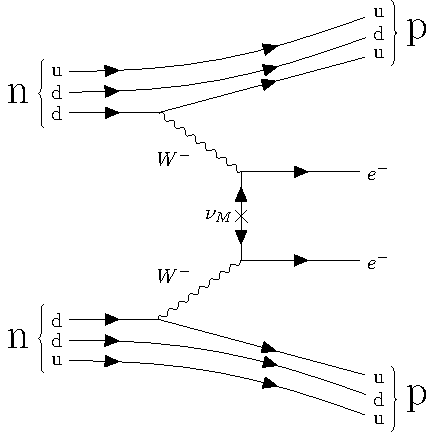
\includegraphics[width=0.55\linewidth]{figures/0vbb.pdf}
    \caption{Feynman diagram for a neutrinoless double beta decay interaction, emitting two electron in the final state and no neutrinos.}
    \label{fig:0vbb}
\end{figure}

This process would also violate the lepton number with $\Delta L = 2$. In this case, the PMNS matrix in eq. \eqref{eq:pmns} acquires two extra Majorana phases in the form:
\begin{equation}
    U_{PMNS}^M = U_{PMNS} \begin{bmatrix}
    e^{i\alpha} & 0 & 0 \\
    0 & e^{i\beta} & 0 \\
    0 & 0 & 1
    \end{bmatrix}.
\end{equation}

Several experiments are actively looking or planning to look for $0\nu\beta\beta$ decays, using $^{130}$Te (CUORE, SNO+), $^{136}$Xe (KamLAND-Zen, EXO, NEXT), or $^{76}$Ge (GERDA). 
The KamLAND-Zen collaboration measured the lower limit for $0\nu\beta\beta$ decay half-life at $T_{\frac{1}{2}} > 1.07\times10^{26}$~years, which corresponds to an effective Majorana mass of 61-165 meV \cite{KamLAND-Zen:2016pfg}.

\subsection{The Seesaw mechanism}
A process which could explain the small masses of the neutrinos, compared to the other fermions, is the so-called \emph{seesaw} mechanism, which here we describe using the approach in \cite{Grossman:2003eb}. 
The most general Lagrangian with right-handed neutrinos can be written as:

\begin{align}
    -2\mathcal{L}_{\mathrm{mass}} & = \mathcal{L}^D_L + \mathcal{L}^D_R + \mathcal{L}^M_L + \mathcal{L}^M_R + h.c. \\
    & = m_D \bar{\nu}_R \nu_L + m_D \bar{\nu}^C_L\nu^C_R + m_L\bar{\nu}_L^C\nu_L + m_R \bar{\nu}_R^C\nu_R.
\end{align}
This term can be expressed as a matrix equation 
\begin{equation}
    -2\mathcal{L_\mathrm{mass}} = \begin{bmatrix}
    \bar{\nu}_L^C & \bar{\nu}_R
    \end{bmatrix}\begin{bmatrix}
    m_L & m_D \\
    m_D & m_R
    \end{bmatrix}\begin{bmatrix}
    \nu_L \\ \nu_R^C
    \end{bmatrix},
\end{equation}
where $m_D$ is the Dirac mass term and $m_L$ ($m_R$) is the Majorana mass term for the left-handed (right-handed) component. 

Since the SM forbids the left-handed Majorana term (it is not gauge invariant), it is possible to set $m_L=0$. For large values of $m_R$, the eigenvalues of the mass matrix are:
\begin{align}
    m_1 & = \frac{m_D^2}{m_R} \\
    m_2 & = m_R \left(1+\frac{m_D^2}{m_R^2}\right) \approx m_R
\end{align}. With a value of $m_R$ at the GUT scale, this would \emph{naturally} give a small value for the neutrino masses. 

The existence of heavy Majorana neutrinos is closely related to the \emph{leptogenesis} hypothesis. In this scenario, the heavy Majorana neutrinos present in the early universe would have decayed into leptons (or antileptons) and Higgs bosons. The so-called \emph{sphaleron} processes would then convert the leptons into baryons and the presence of CP violation in this heavy neutrino sector would then explain the matter-antimatter asymmetry in the universe. It is worth mentioning that this model satisfies the Sakharov conditions \cite{Sakharov:1967dj} for baryogenesis, since it presents baryon number violation, CP violation, and out-of-equilibrium interactions \cite{DiBari:2012fz}.


\section{Neutrino interaction modes}\label{sec:modes}
The interaction between the neutrino and the nucleon can have different forms and a good understanding of their phenomenology is of fundamental importance for the success of any neutrino experiment.
Figure \ref{fig:ccqecross} shows the neutrino cross-section for charged-current interactions divided into three main interaction modes: quasi-elastic (QE), resonant (RES), and deep inelastic scattering (DIS). 

\begin{figure}[htbp]
    \centering
    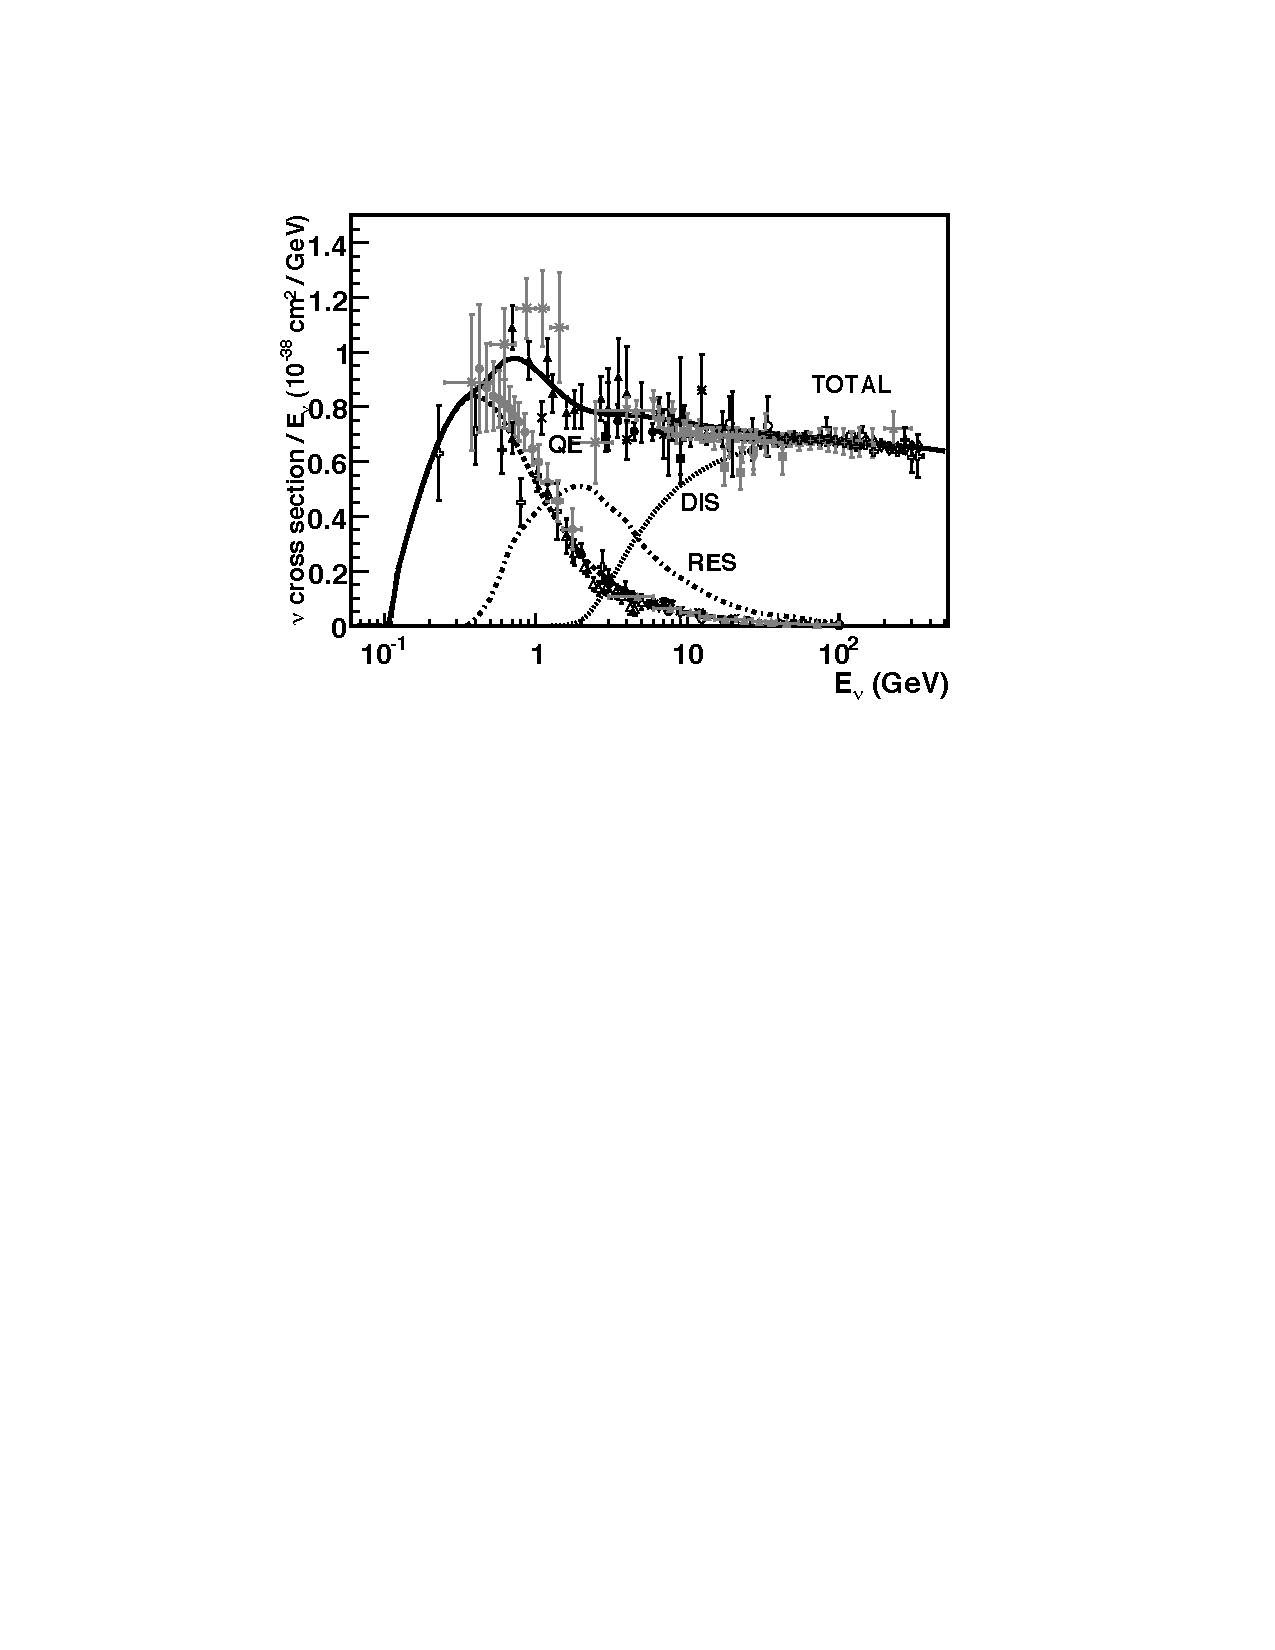
\includegraphics[width=0.7\linewidth]{figures/ccqecross.pdf}
    \caption{Total neutrino per nucleon charged-current cross section (for an isoscalar target) divided by neutrino energy and plotted as a function of energy. Adapted from \cite{Formaggio:2013kya}.}
    \label{fig:ccqecross}
\end{figure}

\begin{description}
\item[Quasi-elastic interaction.] In a charged-current quasi-elastic interaction, the neutrino exchange a $W$ boson with a single nucleon, which is knocked out and leaves a \emph{hole} in the nucleus. Hence its name 1p-1h (one particle, one hole). In this case, the incident neutrino does not have enough energy to break up or excite the nucleus. This is the dominant interaction in the sub-GeV energy range. Figure \ref{fig:ccqe_feyn} shows the Feynman diagram for a CCQE neutrino-nucleus interaction.

The simulation used in this document employs the GENIE neutrino generator, set up to use the Llewellyn-Smith parametrisation for the CCQE interactions \cite{LlewellynSmith:1971uhs} and the Relativistic Fermi Gas model for the nucleus.
In this model, the interaction is calculated with the impulse approximation (IA): the neutrino interacts with only one nucleon, which can have short-range correlations with other nucleons (\emph{bound but independent}).

However, hadrons exiting the nucleus can re-interact and change identity or eject other hadrons (Final State Interactions, FSI), so it is possible to have a CCQE interaction with no protons or with a pion in the final state. It is also possible to have multinucleon excitations, mainly through the so-called meson exchange current (MEC). This interaction is responsible for np-nh events, where more than one nucleon is emitted.

The neutral-current equivalent of a CCQE interaction is neutral-current elastic scattering (NCE), which typically ejects a nucleon.

At low exchanged momentum $Q^2$ the neutrino can also scatter elastically with the entire nucleus (coherent elastic neutrino-nucleus) scattering, CE$\nu$NS), as recently detected by the COHERENT collaboration \cite{Akimov:2017ade}. In this case, the nucleus remains in its initial state and its small recoil represents the only observable.

\begin{figure}[htbp]
    \centering
    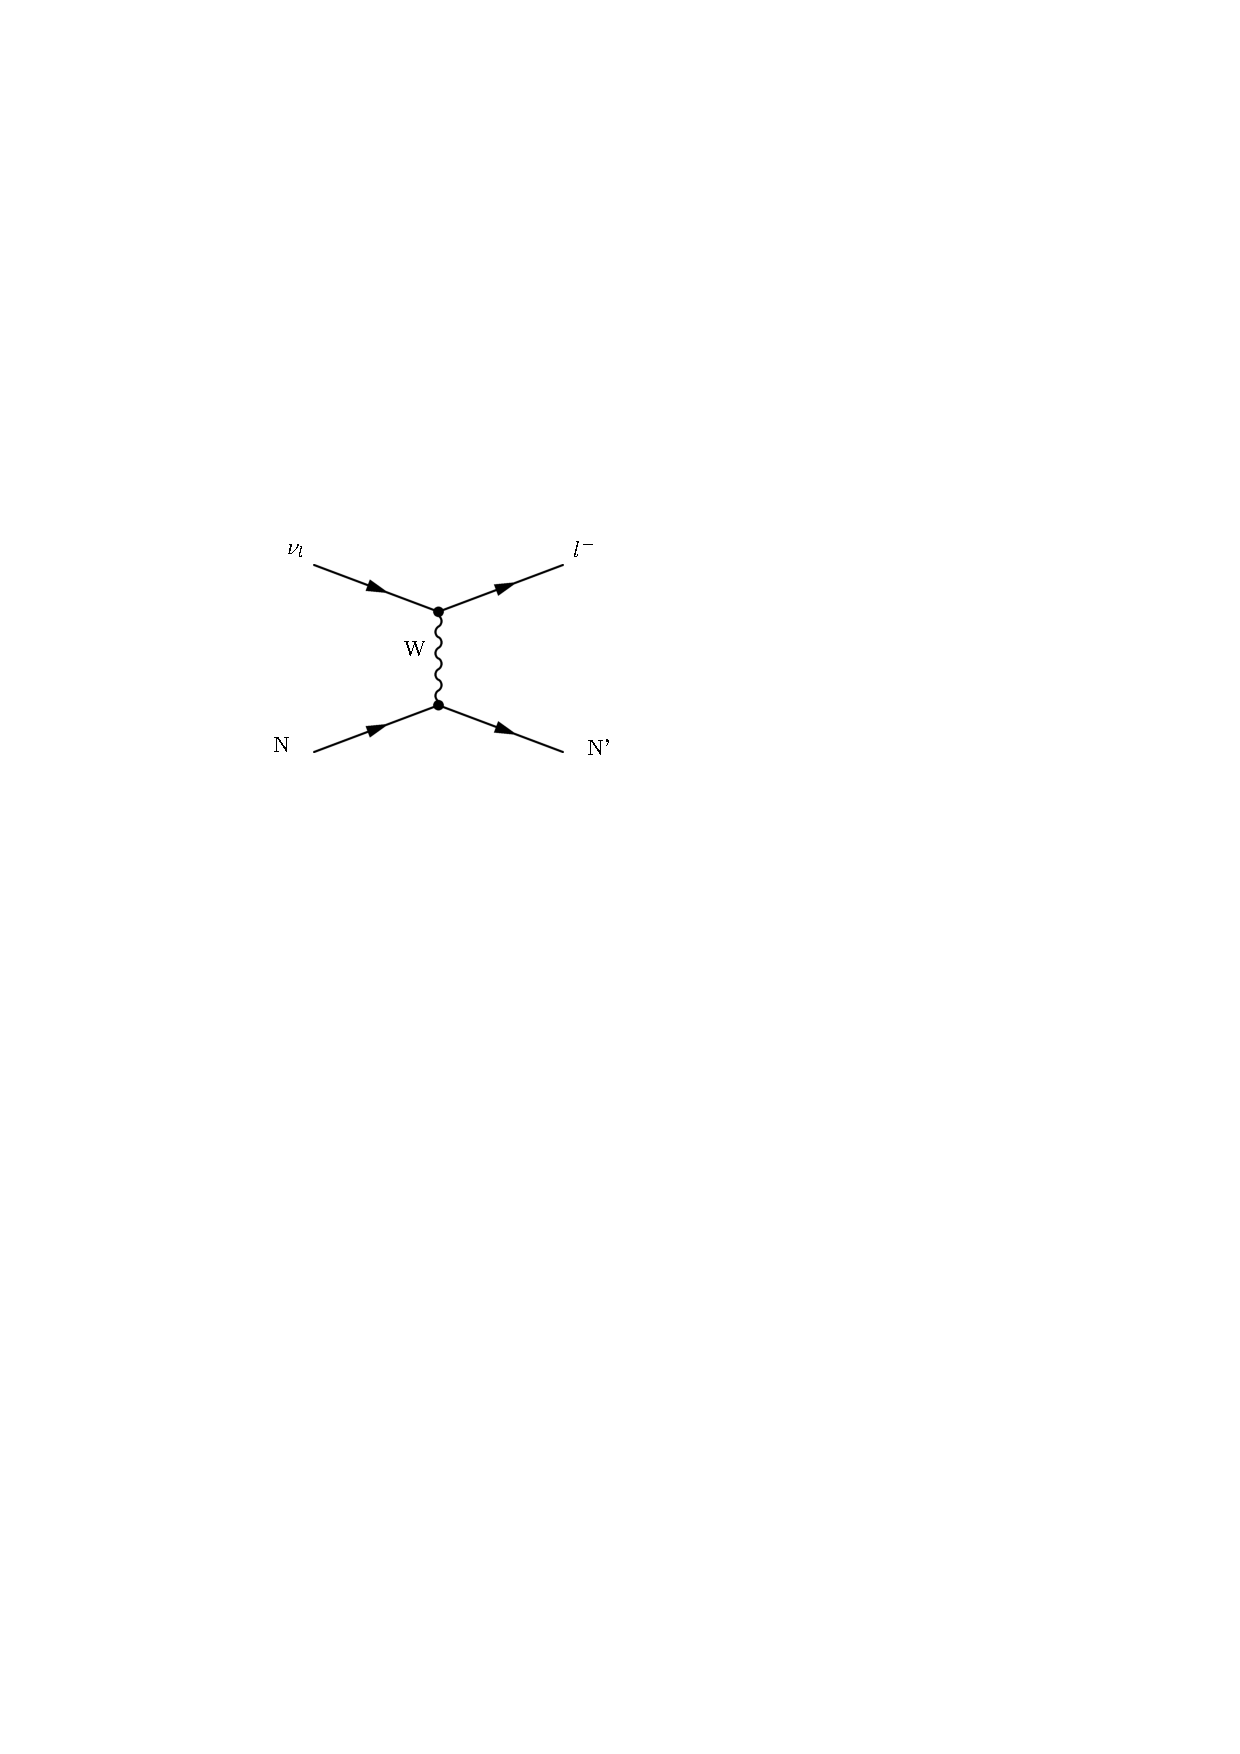
\includegraphics[width=0.65\linewidth]{figures/ccqe_feyn.pdf}
    \caption{Feynman diagram of a charged-current quasi-elastic neutrino-nucleon interaction.}
    \label{fig:ccqe_feyn}
\end{figure}

\item[Resonant and coherent interactions.] In a resonant interaction, the neutrino has enough energy to excite the nucleon to form a resonance, which rapidly decays to a nucleon and one or more mesons while still in the nucleus, as in:
\begin{align}
&\nu_l + p \rightarrow \Delta^{++} \rightarrow l^- + \pi^+ + p \\
&\nu_l + n \rightarrow \Delta^{+} \rightarrow l^- + \pi^+ + n.
\end{align}
This interaction is allowed both by charged current and neutral current exchange.

The GENIE setup used here employs the Rein-Sehgal model for the resonance production and the Bodek-Ritchie RFG model for the interaction of the nucleon within the nucleus. Also in this case, the FSI can cause the absorption of the pion in the nucleus or exchange the charge of the pion.

At low $Q^2$, pions can be produced also in coherent neutrino-nucleus processes, where the nucleus is left unchanged and a pion is emitted, as shown in the Feynman diagram of Figure \ref{fig:ccoh_feyn}.

\begin{figure}[htbp]
  \begin{subfigure}{0.48\textwidth}
    \begin{center}
    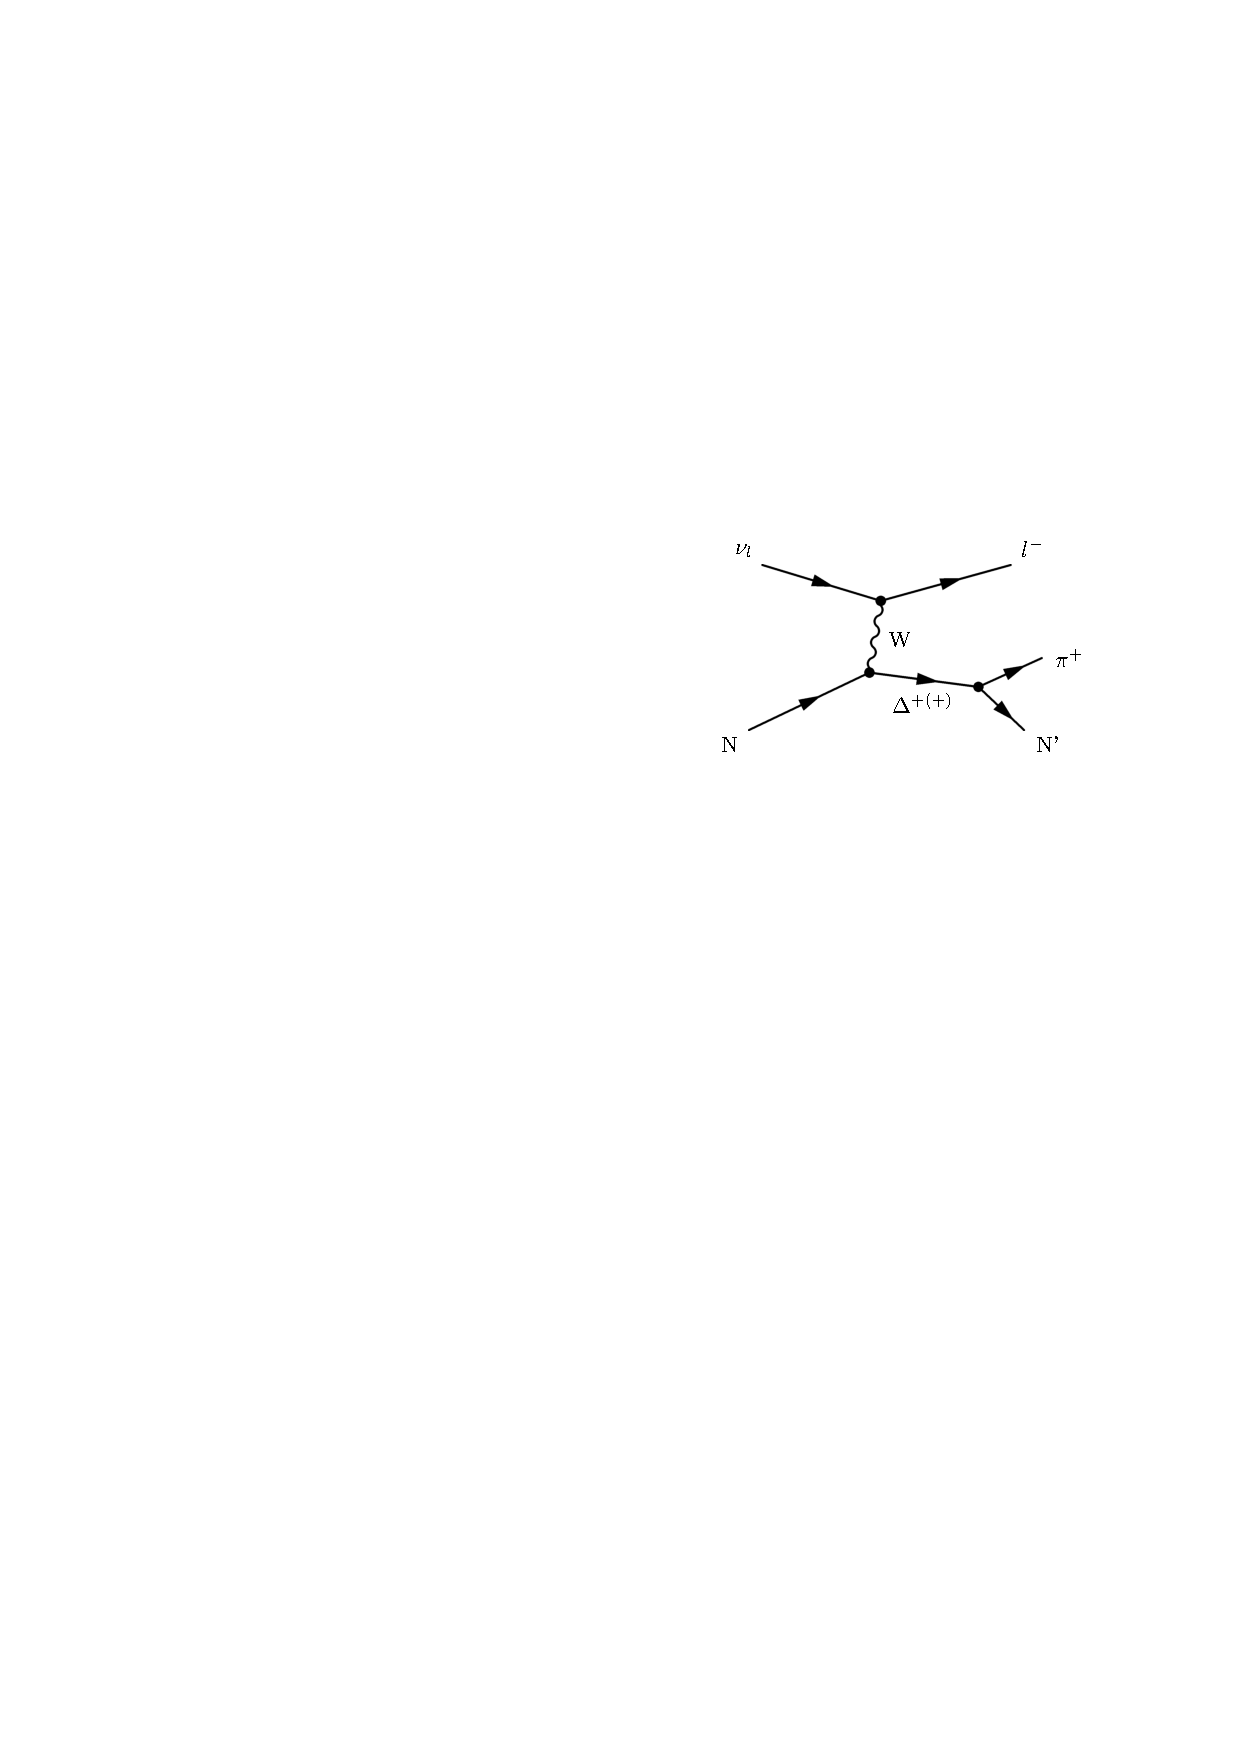
\includegraphics[width=\linewidth]{figures/ccres_feyn.pdf}
    \caption{Charged-current resonant interaction.}
    \label{fig:ccres_feyn}
    \end{center}
  \end{subfigure}\hfill
  \begin{subfigure}{0.48\textwidth}
    \begin{center}
    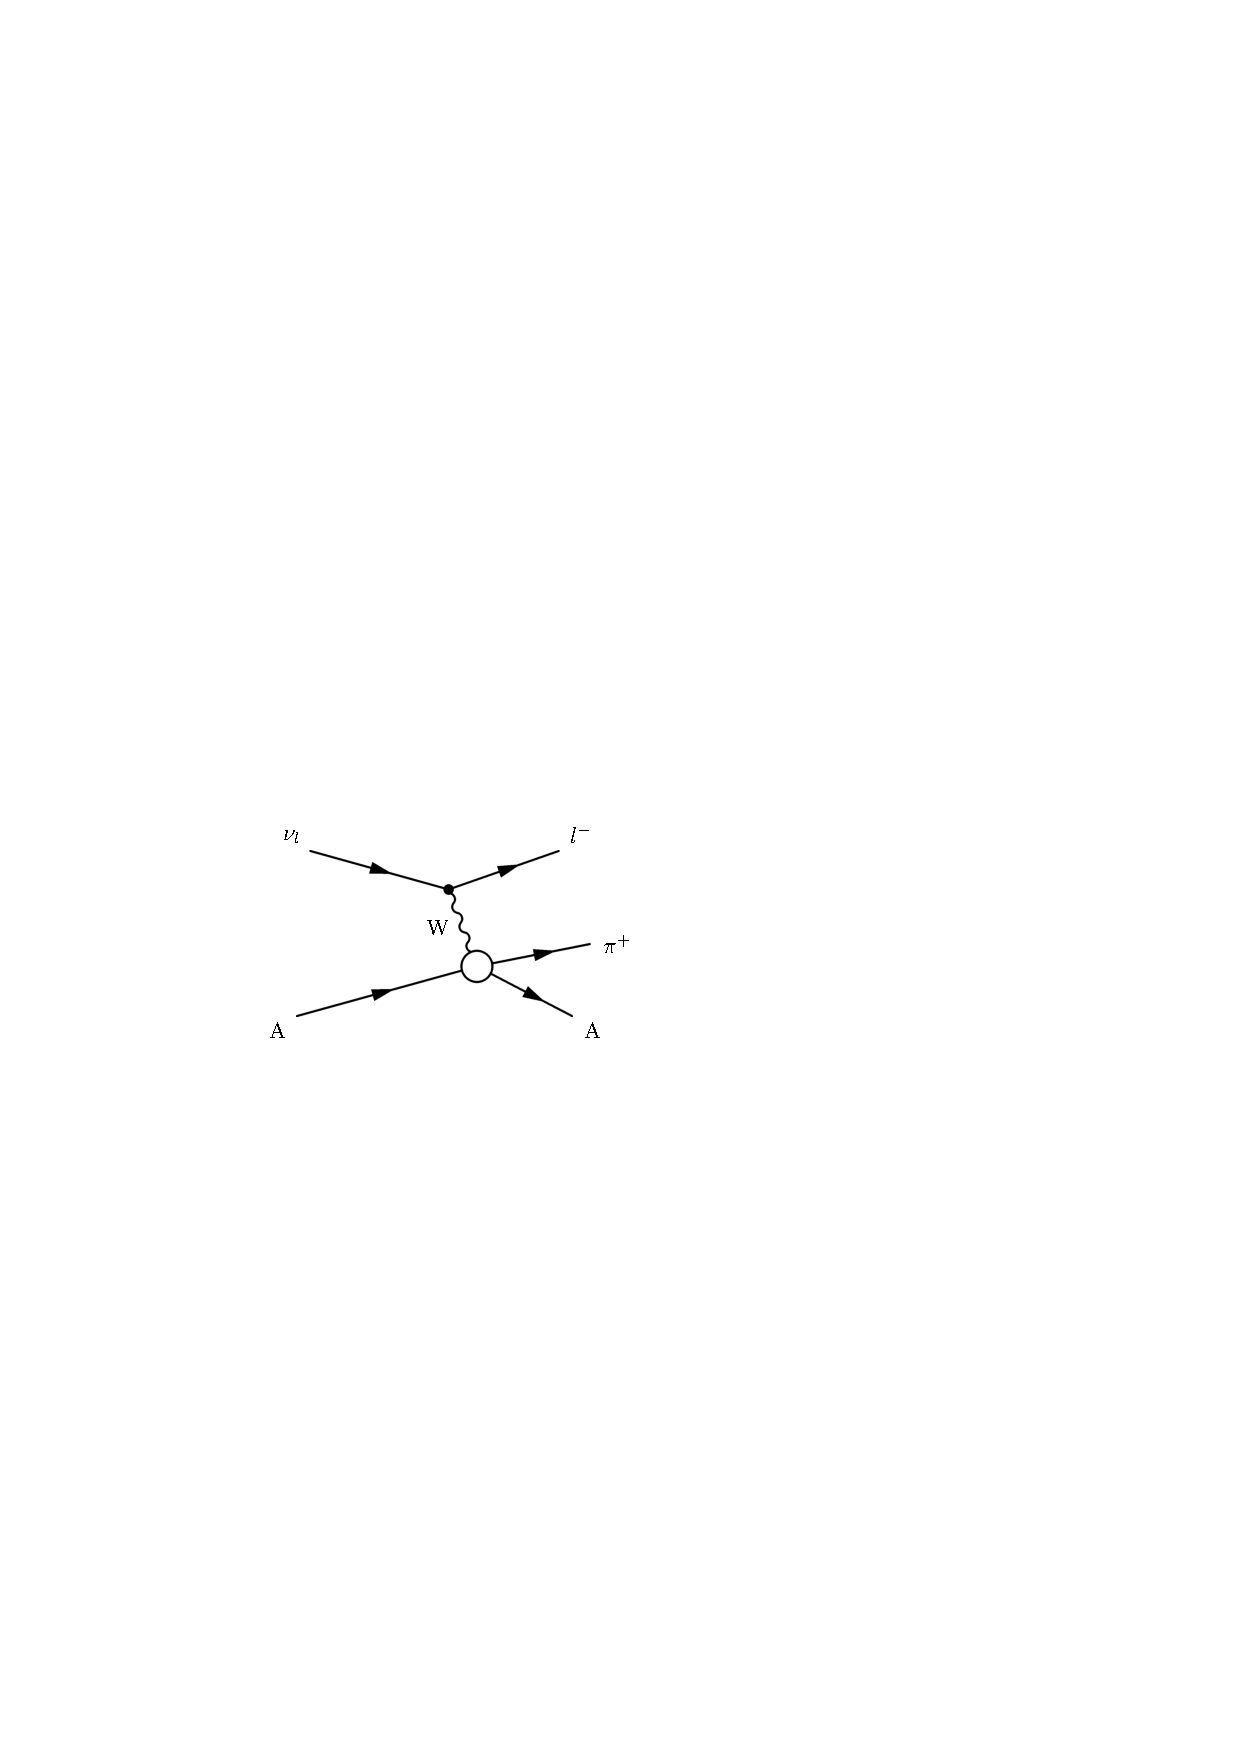
\includegraphics[width=\linewidth]{figures/ccoh_feyn.pdf}
    \caption{Charged-current coherent interaction.}
    \label{fig:ccoh_feyn}
    \end{center}
  \end{subfigure}
  \caption{Feynman diagrams of two neutrino interactions which can produce pions in the final state, charged-current resonant (left) and charged-current coherent (right).}
\end{figure}

\item[Deep inelastic scattering.] In this case, the neutrino has enough energy to interact with the single nucleon components, the quarks, and to break up the nucleus. The result of this interaction often consists in several mesons in the final state. This is the dominant interaction mode for high-energy neutrinos ($>5$~GeV). It is simulated by our setup of GENIE using the Bodek-Yang model.

Figure \ref{fig:ccdis_feyn} shows the Feynman diagram for this kind of interaction.

\begin{figure}[htbp]
    \centering
    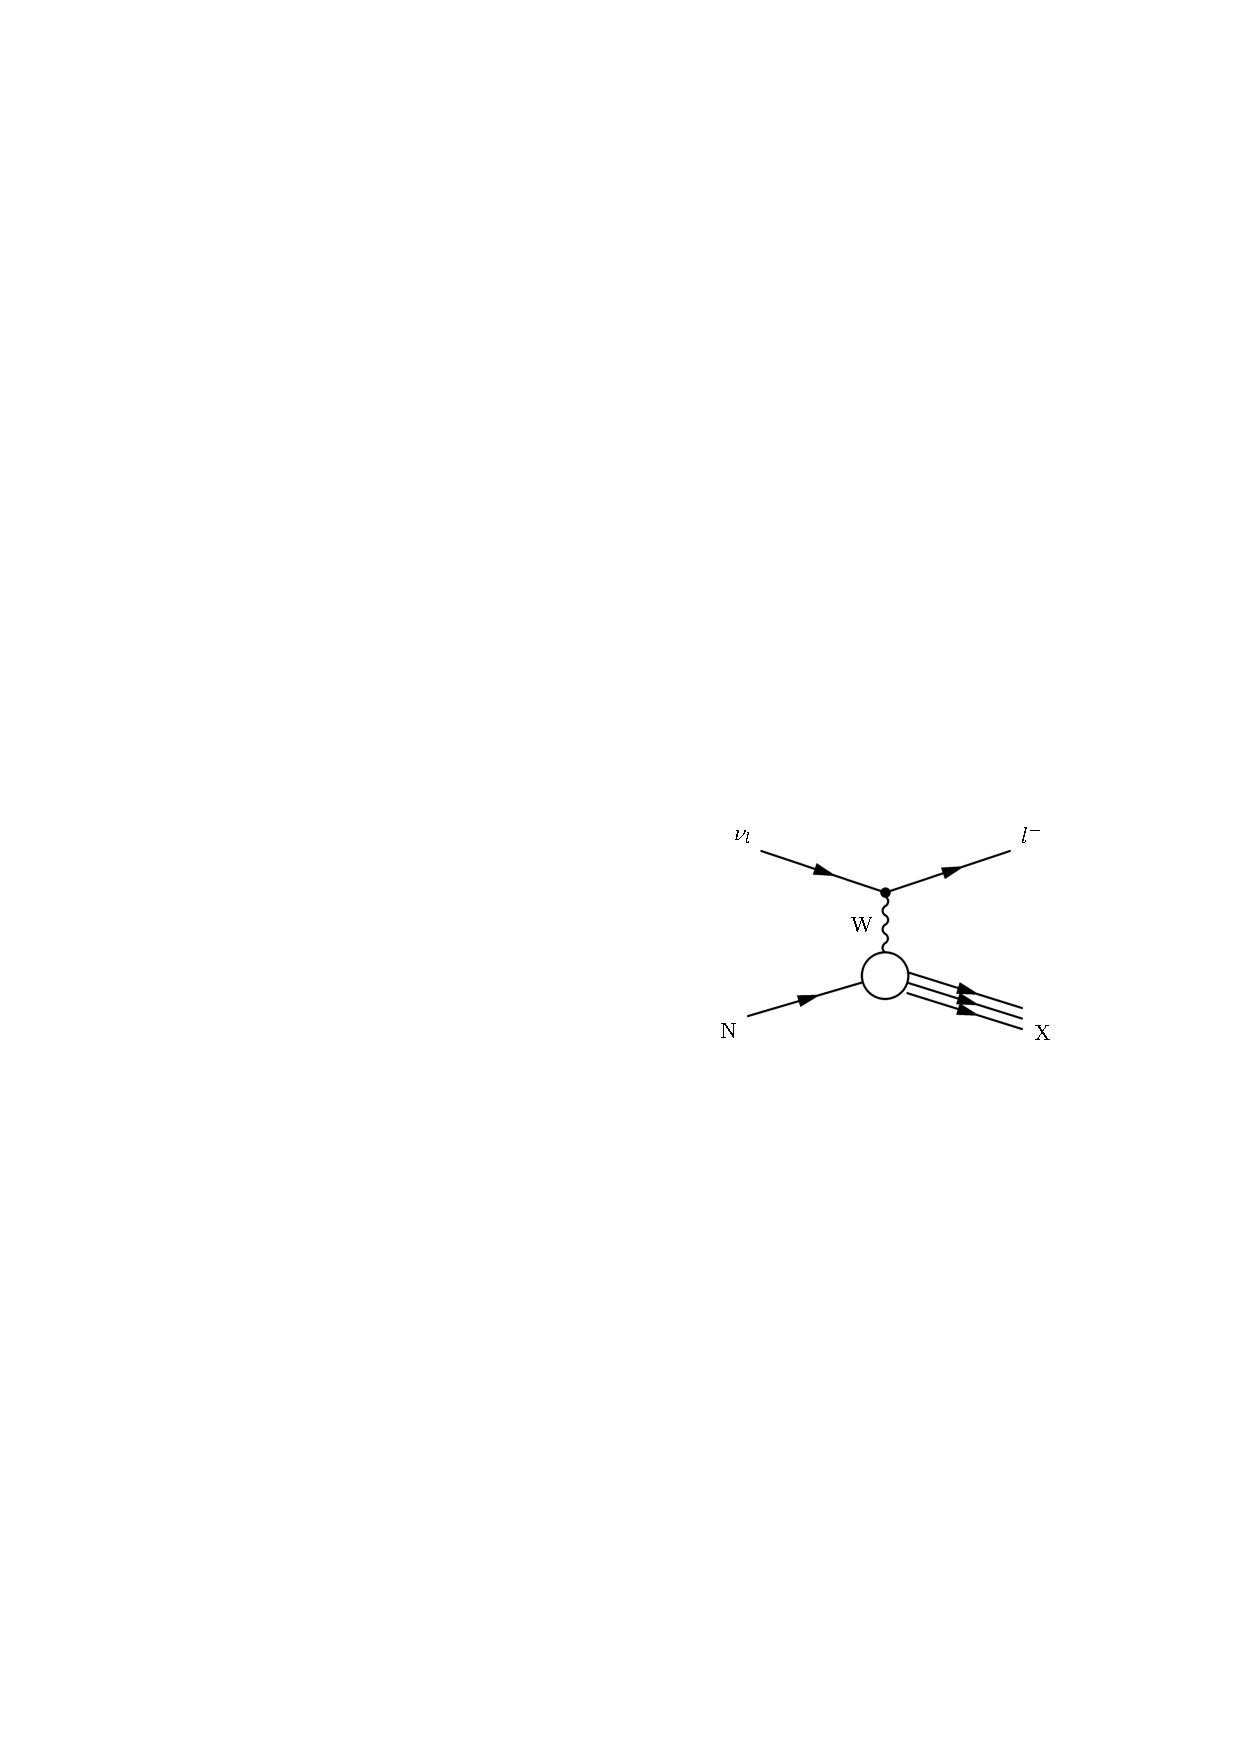
\includegraphics[width=0.65\linewidth]{figures/ccdis_feyn.pdf}
    \caption{Feynman diagram of a charged-current deep inelastic scattering neutrino-nucleon interaction.}
    \label{fig:ccdis_feyn}
\end{figure}


\end{description}

This rich scenario makes the correct reconstruction of neutrino interactions very challenging for any experiment. Usually, oscillations experiments like MiniBooNE (see Section \ref{sec:miniboone}) look for CCQE interactions, whose signature in the detector is easier to identify, but which also require a precise assessment of the final-state interactions.

\section{Conclusions}
Several experiments have shown compelling evidence for neutrino oscillations, which in turn require non-null neutrino masses. At the moment, massive neutrinos represent the only portal into BSM physics and, for this reason, neutrino physics is one of the most active sectors in particle physics. In the last decade, the parameters of the PMNS mixing matrix have been constrained to a precision smaller than 5\%, but some neutrino properties still need to measured. In particular, the CP-violating phase, the neutrino mass hierarchy, and the Majorana or Dirac nature of the neutrino are all research topics actively investigated both by present and future experiments. 